\documentclass[conference]{styles/acmsiggraph}

\usepackage{comment} % enables the use of multi-line comments (\ifx \fi)
\usepackage{lipsum} %This package just generates Lorem Ipsum filler text.
\usepackage{fullpage} % changes the margin
\usepackage{enumitem} % for customizing enumerate tags
\usepackage{amsmath,amsthm,amssymb}
\usepackage{listings}
\usepackage{graphicx}
\usepackage{etoolbox}   % for booleans and much more
\usepackage{verbatim}   % for the comment environment
\usepackage[dvipsnames]{xcolor}
\usepackage{fancyvrb}
\usepackage{hyperref}
\usepackage{menukeys}
\usepackage{titlesec}
\setlength{\parskip}{.8mm}
\usepackage{siunitx}
\usepackage{pdfpages}


\newtheorem{theorem}{Theorem}
\newtheorem{corollary}{Corollary}
\newtheorem{lemma}{Lemma}
\newtheorem{definition}{Definition}

\title{\huge Artificial Intelligence \\ \LARGE {Summary}}
\author{\Large Christian Schmidt \\ \Large Guido Battiston}
\pdfauthor{Christian Schmidt}

\hypersetup{
	colorlinks=true,
	urlcolor=[rgb]{0.97,0,0.30},
	anchorcolor={0.97,0,0.30},
	linkcolor=[rgb]{0.97,0,0.30},
	filecolor=[rgb]{0.97,0,0.30},
}

% redefine \VerbatimInput
\RecustomVerbatimCommand{\VerbatimInput}{VerbatimInput}%
{fontsize=\footnotesize,
 %
 frame=lines,  % top and bottom rule only
 framesep=2em, % separation between frame and text
 rulecolor=\color{Gray},
 %
 label=\fbox{\color{Black}\textbf{OUTPUT}},
 labelposition=topline,
 %
 commandchars=\|\(\), % escape character and argument delimiters for
                      % commands within the verbatim
 commentchar=*        % comment character
}

% convenient norm symbol
\newcommand{\norm}[1]{\left\lVert#1\right\rVert}
\renewcommand{\vec}[1]{\mathbf{#1}}

\titlespacing*{\section}{0pt}{5.5ex plus 1ex minus .2ex}{2ex}
\titlespacing*{\subsection}{0pt}{3ex}{2ex}

\setcounter{secnumdepth}{4}
\renewcommand\theparagraph{\thesubsubsection.\arabic{paragraph}}
\newcommand\subsubsubsection{\paragraph}

\setlength{\parskip}{0.5em}

% a macro for hiding answers
\newbool{hideanswers}
\setbool{hideanswers}{false}
\newenvironment{answer}{}{}
\ifbool{hideanswers}{\AtBeginEnvironment{answer}{\comment} %
\AtEndEnvironment{answer}{\endcomment}}{}

\newcommand{\points}[1]{\hfill \normalfont{(\textit{#1pts})}}
\newcommand{\pointsin}[1]{\normalfont{(\textit{#1pts})}}

\usepackage{lastpage}
\usepackage{fancyhdr}
\pagestyle{fancy} 
\fancyfoot[CO,CE]{\thepage}

\begin{document}
\maketitle

\tableofcontents
\newpage

\section{BFS and DLS}

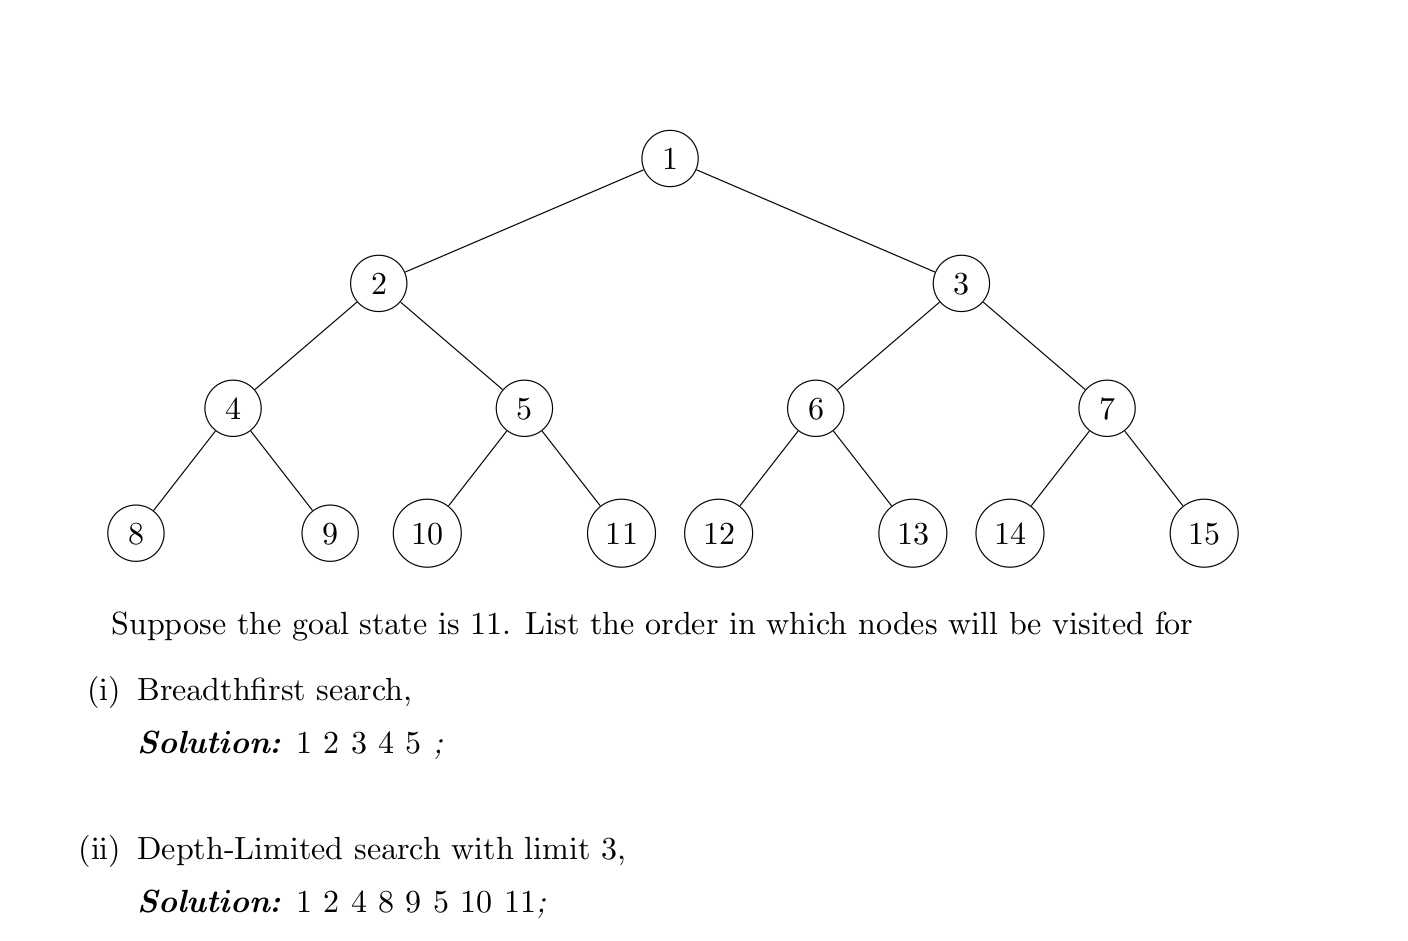
\includegraphics[width=\textwidth]{bfs.png}

\begin{itemize}
    \item \textbf{BFS: goal test is performed at exploration therefore if one of the children is a goal, we abort}
\end{itemize}

\section{Uniform cost search}
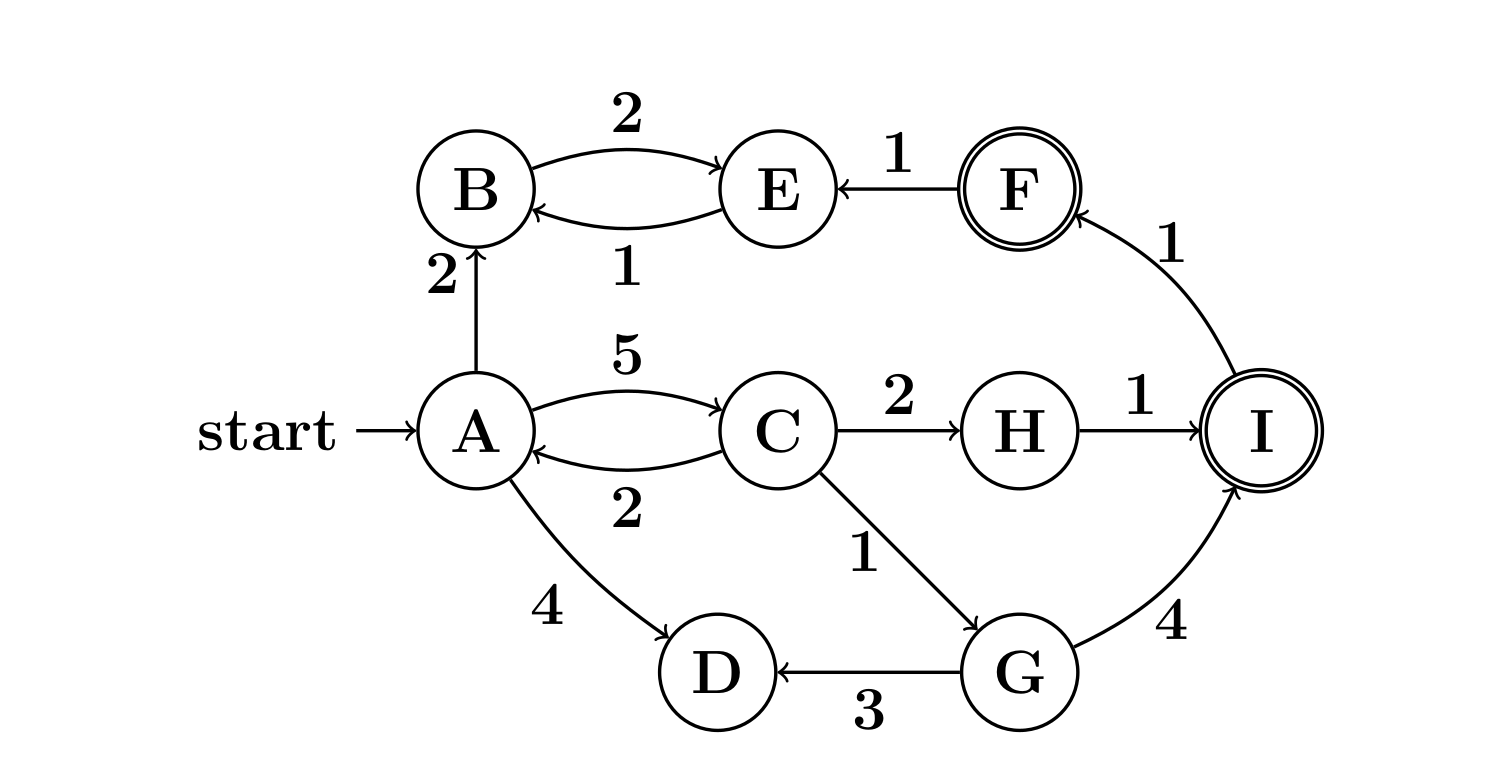
\includegraphics[width=0.5\textwidth]{graph1.png}
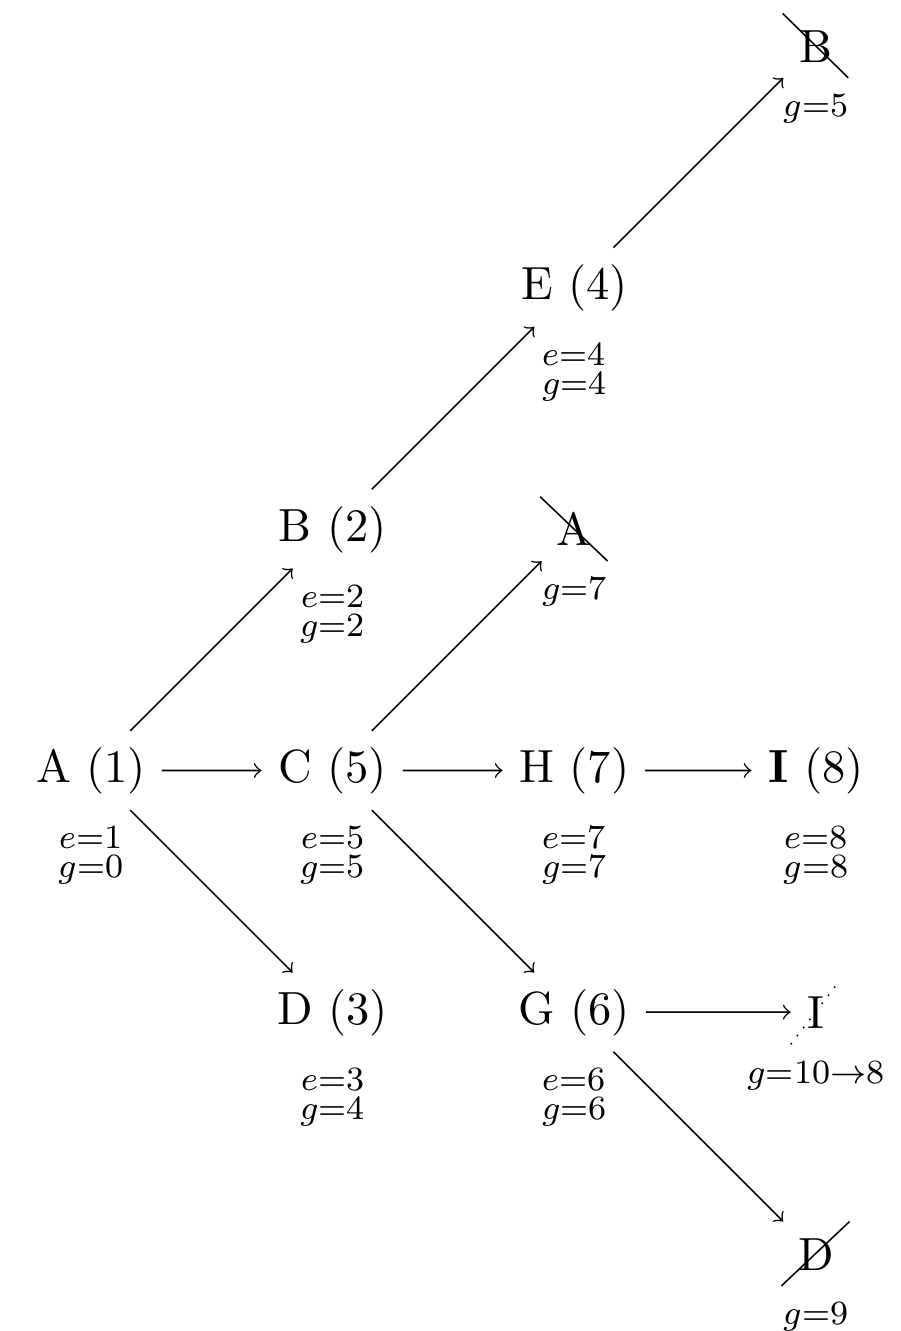
\includegraphics[width=0.5\textwidth]{uniform.png}

\begin{itemize}
    \item goal test at node expansion time
    \item track the priority queue, the path with the lowest cost is taken first
    \item remember to cross out states that are replaced!
    \item mind transitions that go back and forth and also add them to the list when the node is explored
    \item basically A* without h
    \item \textbf{return the optimal path in the end!!!!}
\end{itemize}

\section{Iterative deepening}

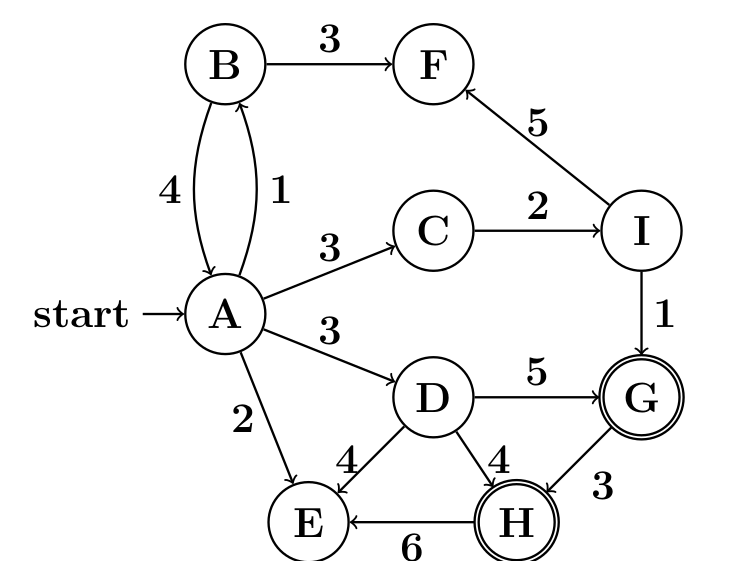
\includegraphics[width=0.4\textwidth]{graph2.png}
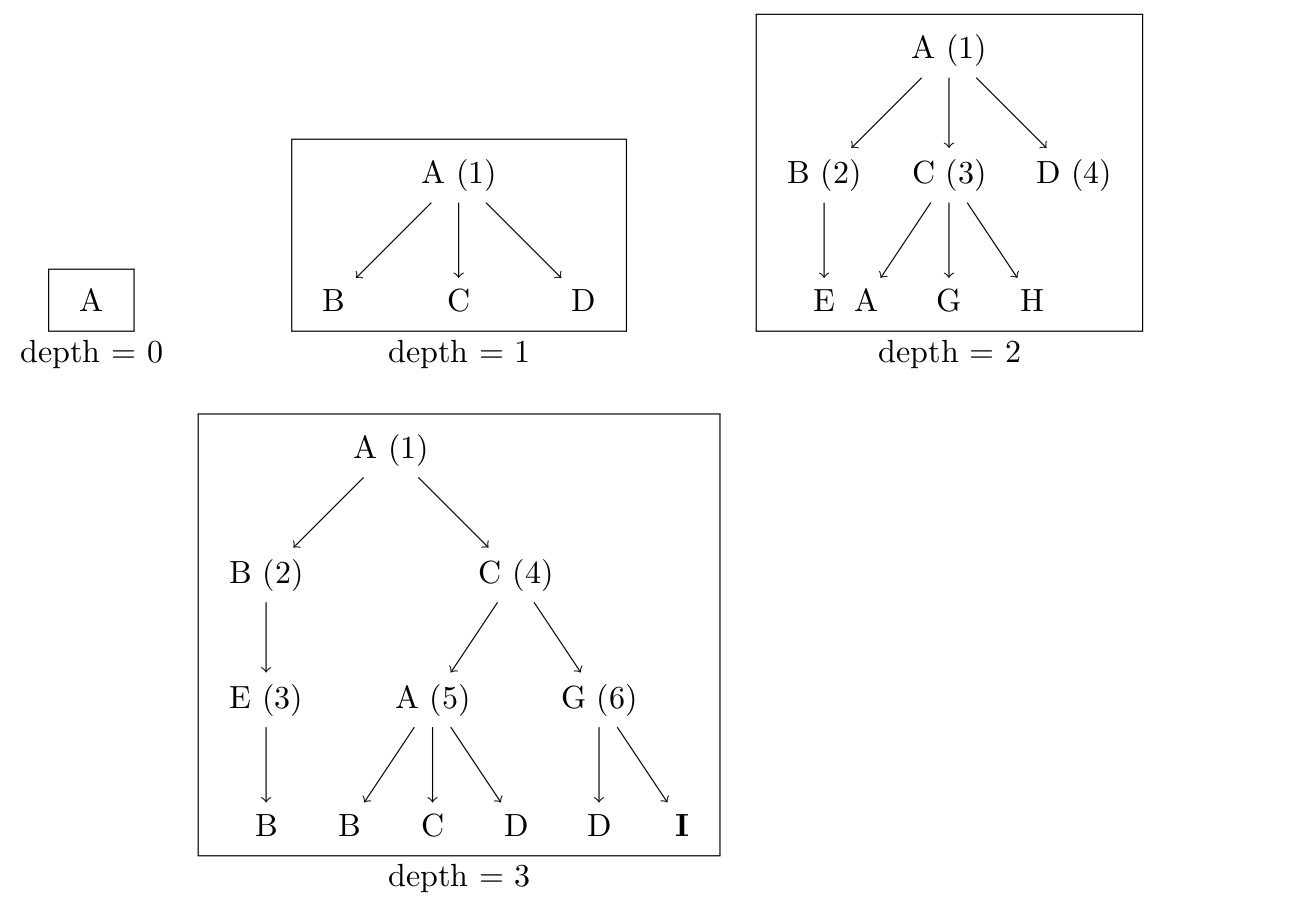
\includegraphics[width=0.7\textwidth]{deepening.png}

\section{Greedy Best First Search}

%TODO

\section{Heuristics}

\subsection{Admissible heuristic}

\begin{itemize}
    \item $h((u,v)) = |u-x| + |v - y| \; \quad (Manhatten \, distance)$ 
    %TODO add more
\end{itemize}

\subsection{Non-Admissible heuristic}
\begin{itemize}
    \item 
\end{itemize}

\section{A*}

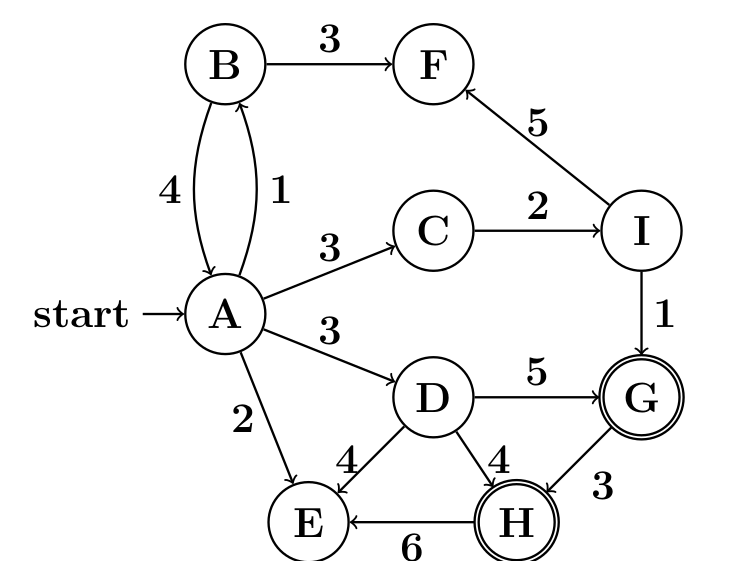
\includegraphics[width=0.3\textwidth]{graph2.png}
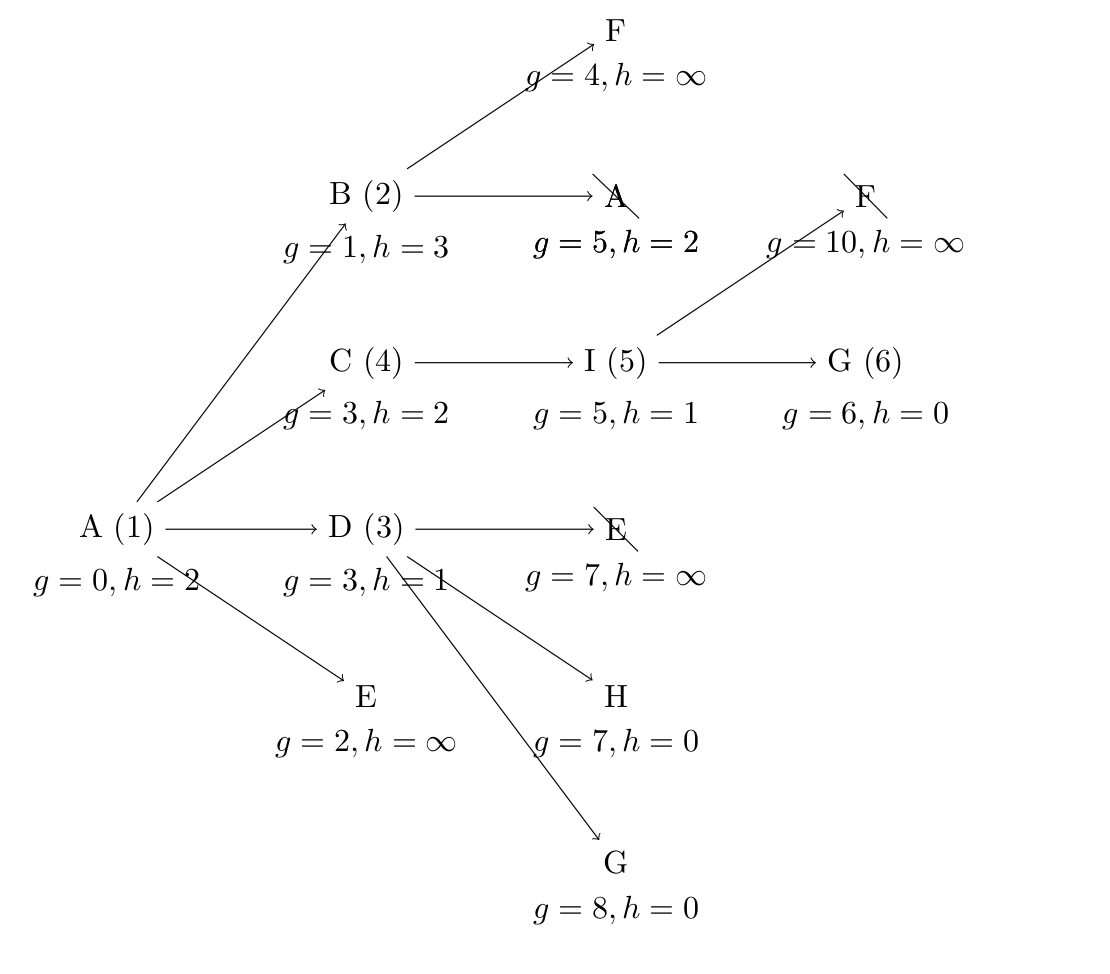
\includegraphics[width=0.7\textwidth]{astar.png}

\begin{itemize}
    \item \textbf{write down the frontier for each exploration step, so write down g+h for all nodes and select the smallest sum}
\end{itemize}

%TODO maybe add pseudocode

\section{UCT Search}

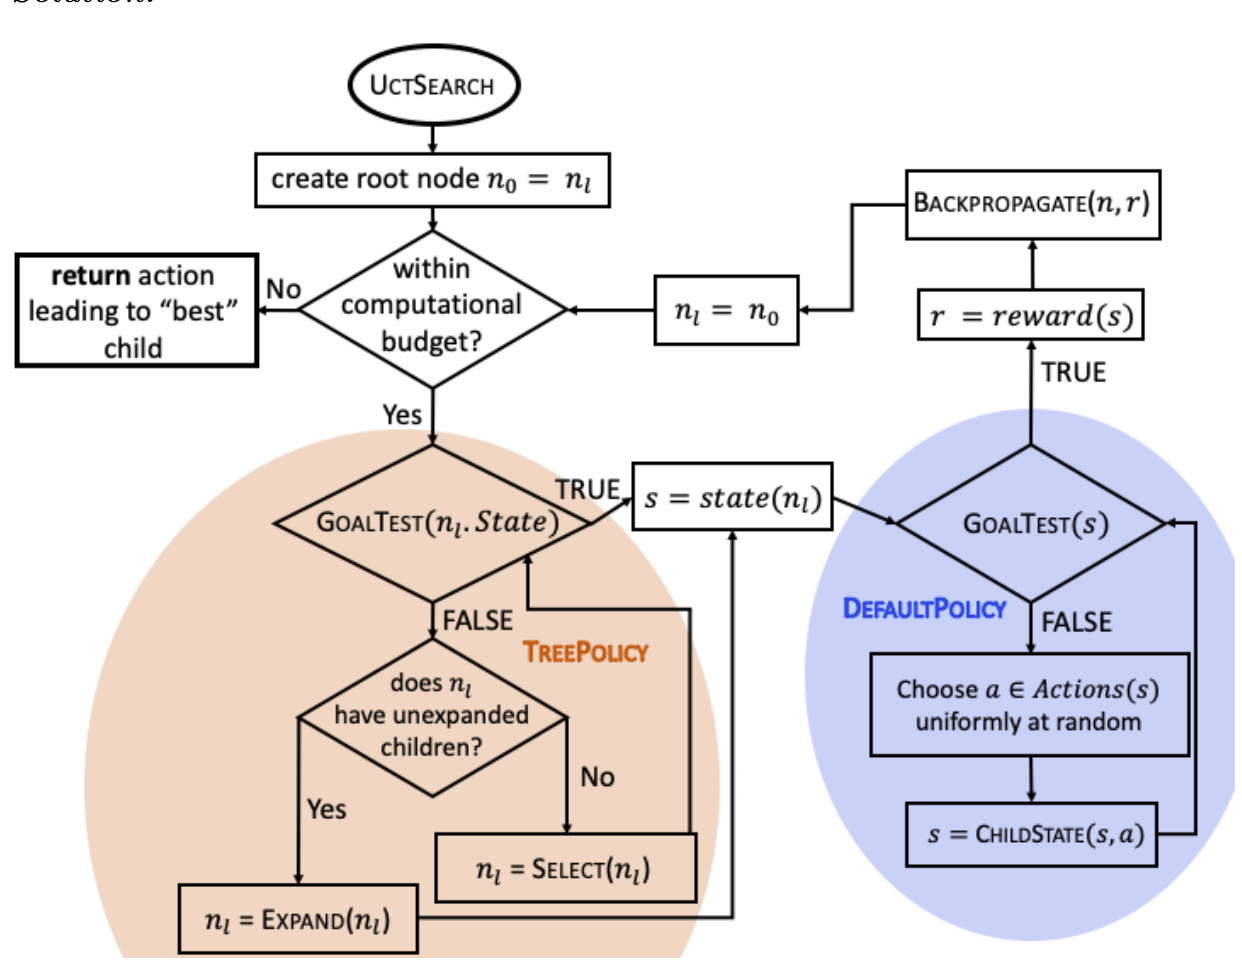
\includegraphics[width=0.7\textwidth]{uct.png}

\pagebreak
\section{Logical formulas}

\subsection{Basics}

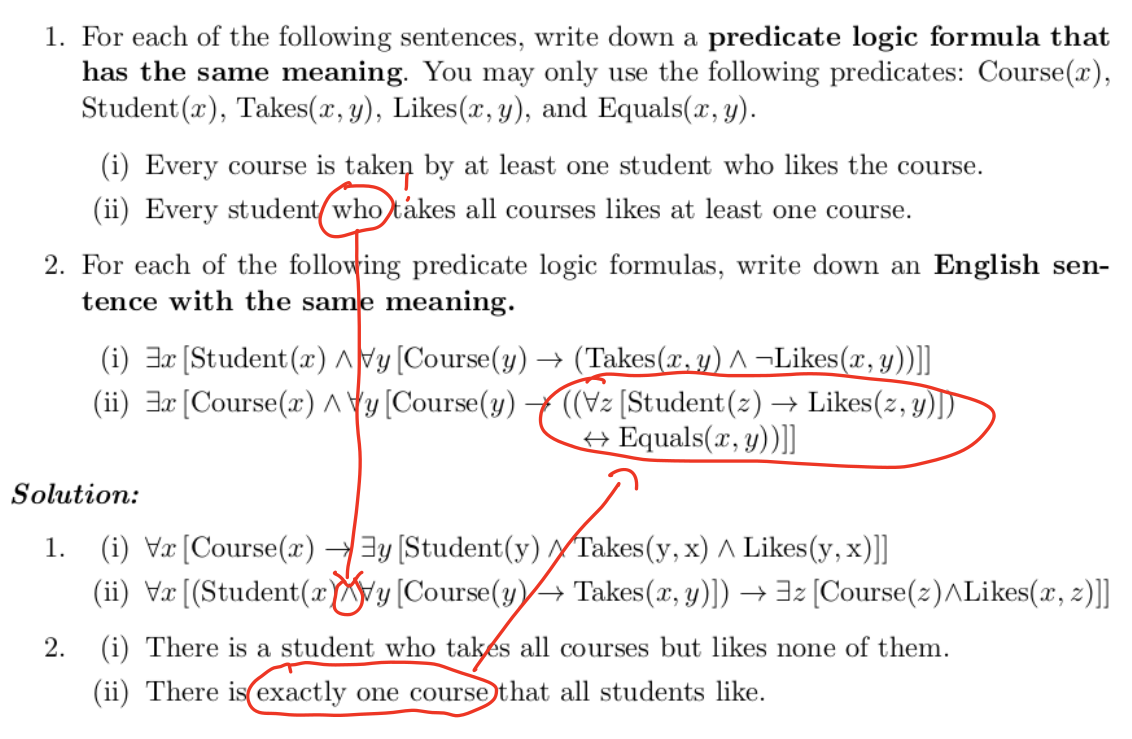
\includegraphics[width=0.8\textwidth]{imgs/basics.png}

\begin{itemize}
    \item When it is a general requirement use $\land$ (e.g. every student), and use $\implies$ when it holds for all instances (e.g. $Course(x) \implies ... $ )
\end{itemize}

\subsection{CNF and DNF transformation}

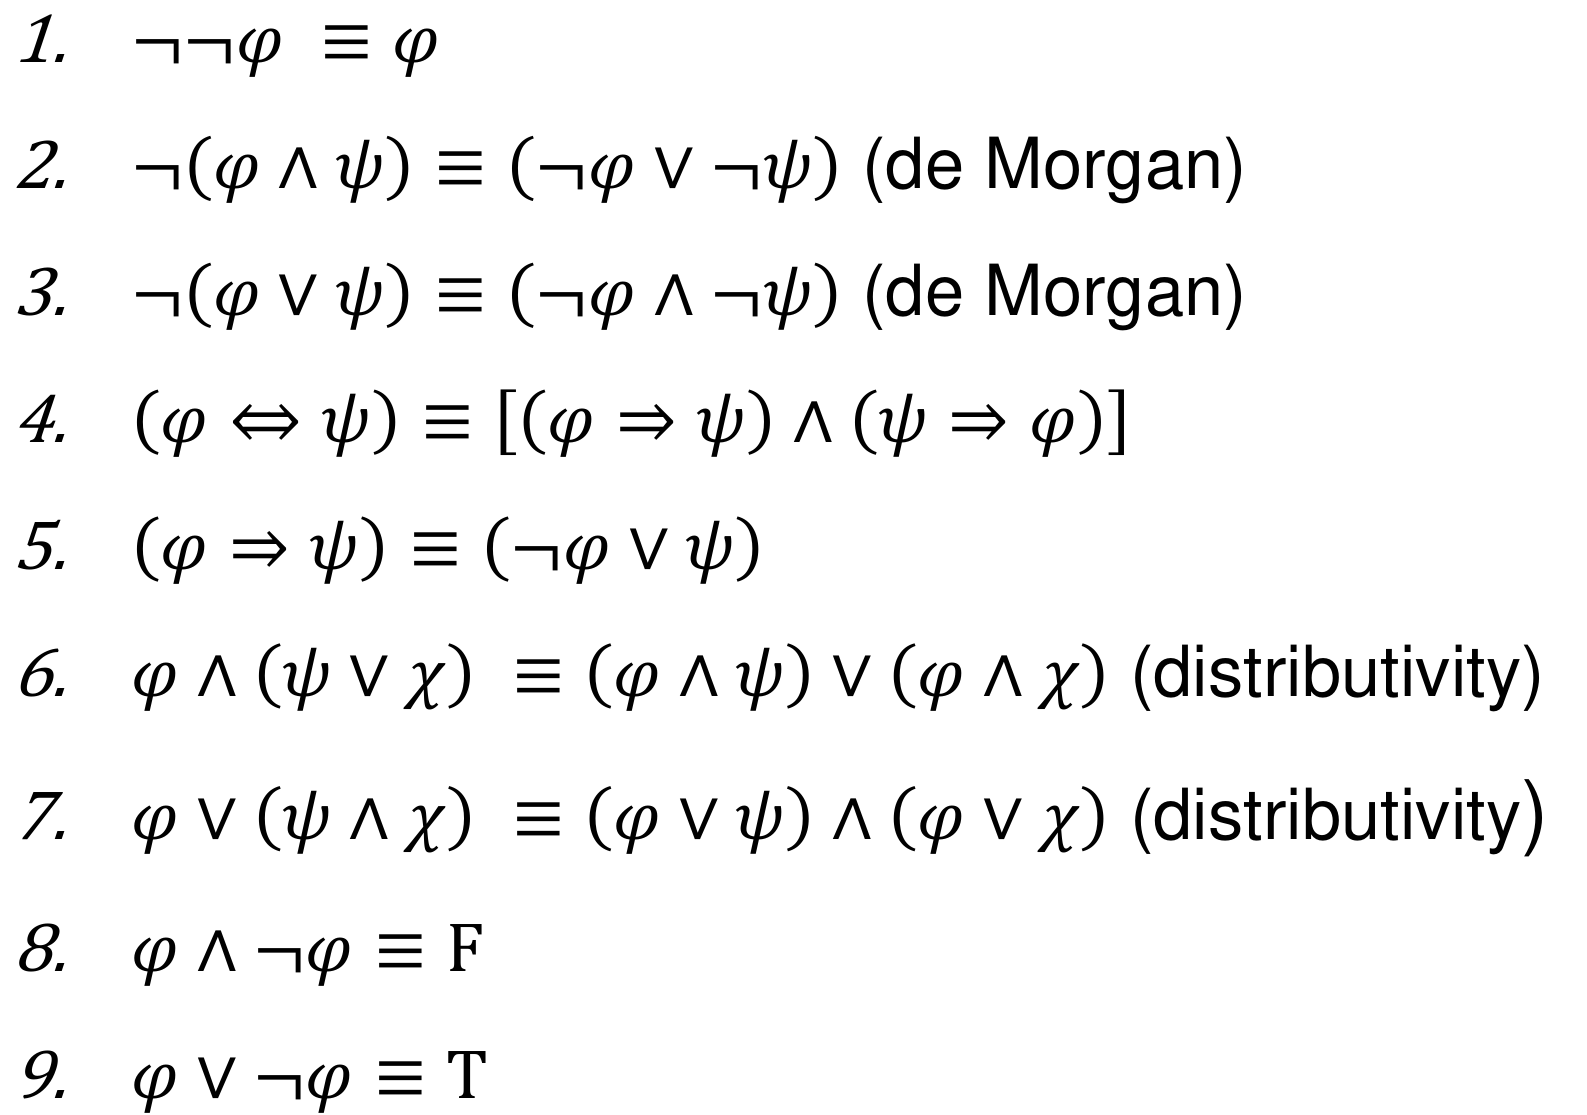
\includegraphics[width=0.5\textwidth]{imgs/transform.png}
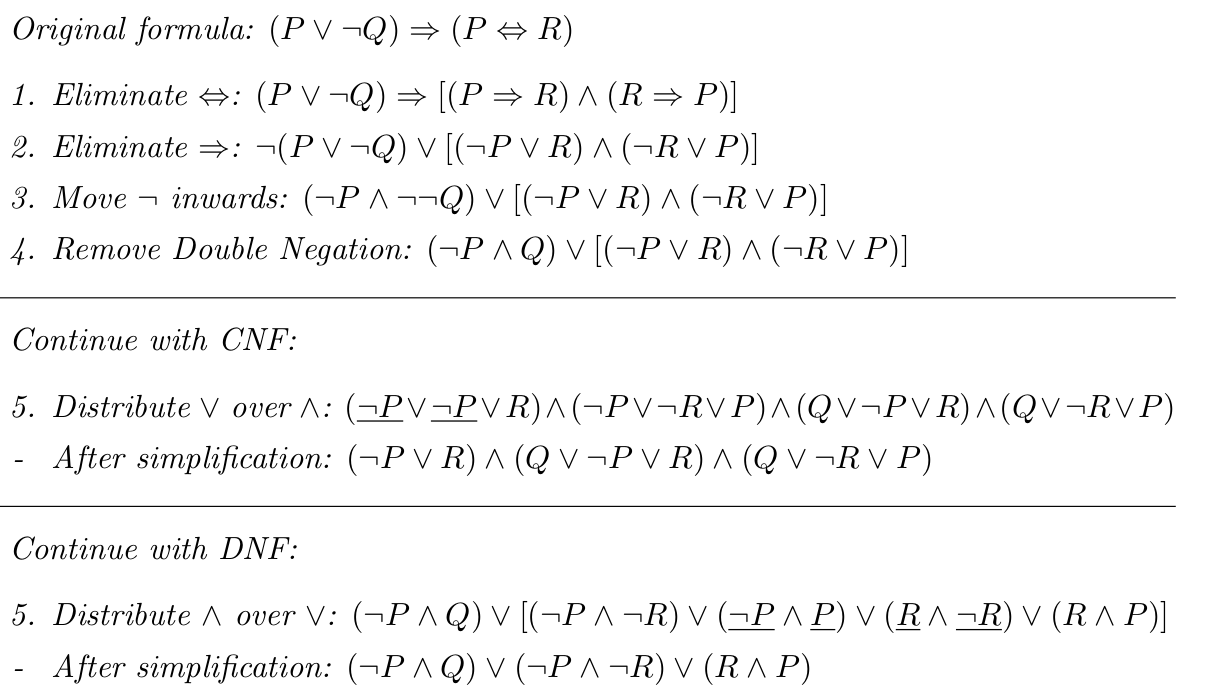
\includegraphics[width=0.8\textwidth]{imgs/transform-example.png}

\subsection{Resolution}

%TODO conflict graph, tutorial slides from , we look what had to happen so that the term could appear (single clause)

To show that something is unsatisfiable:\\
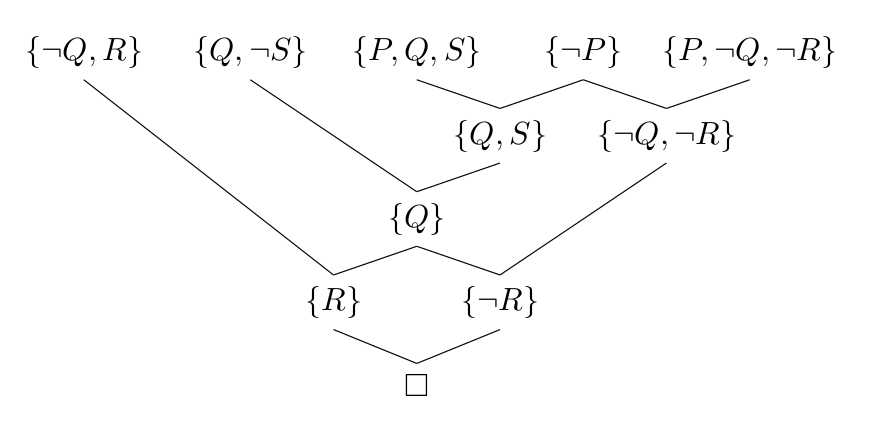
\includegraphics[width=0.8\textwidth]{imgs/resolution.png}\\
If there are complementary literals in two clauses, eliminate them and write the remaining ones in one clause

\subsection{DPLL}

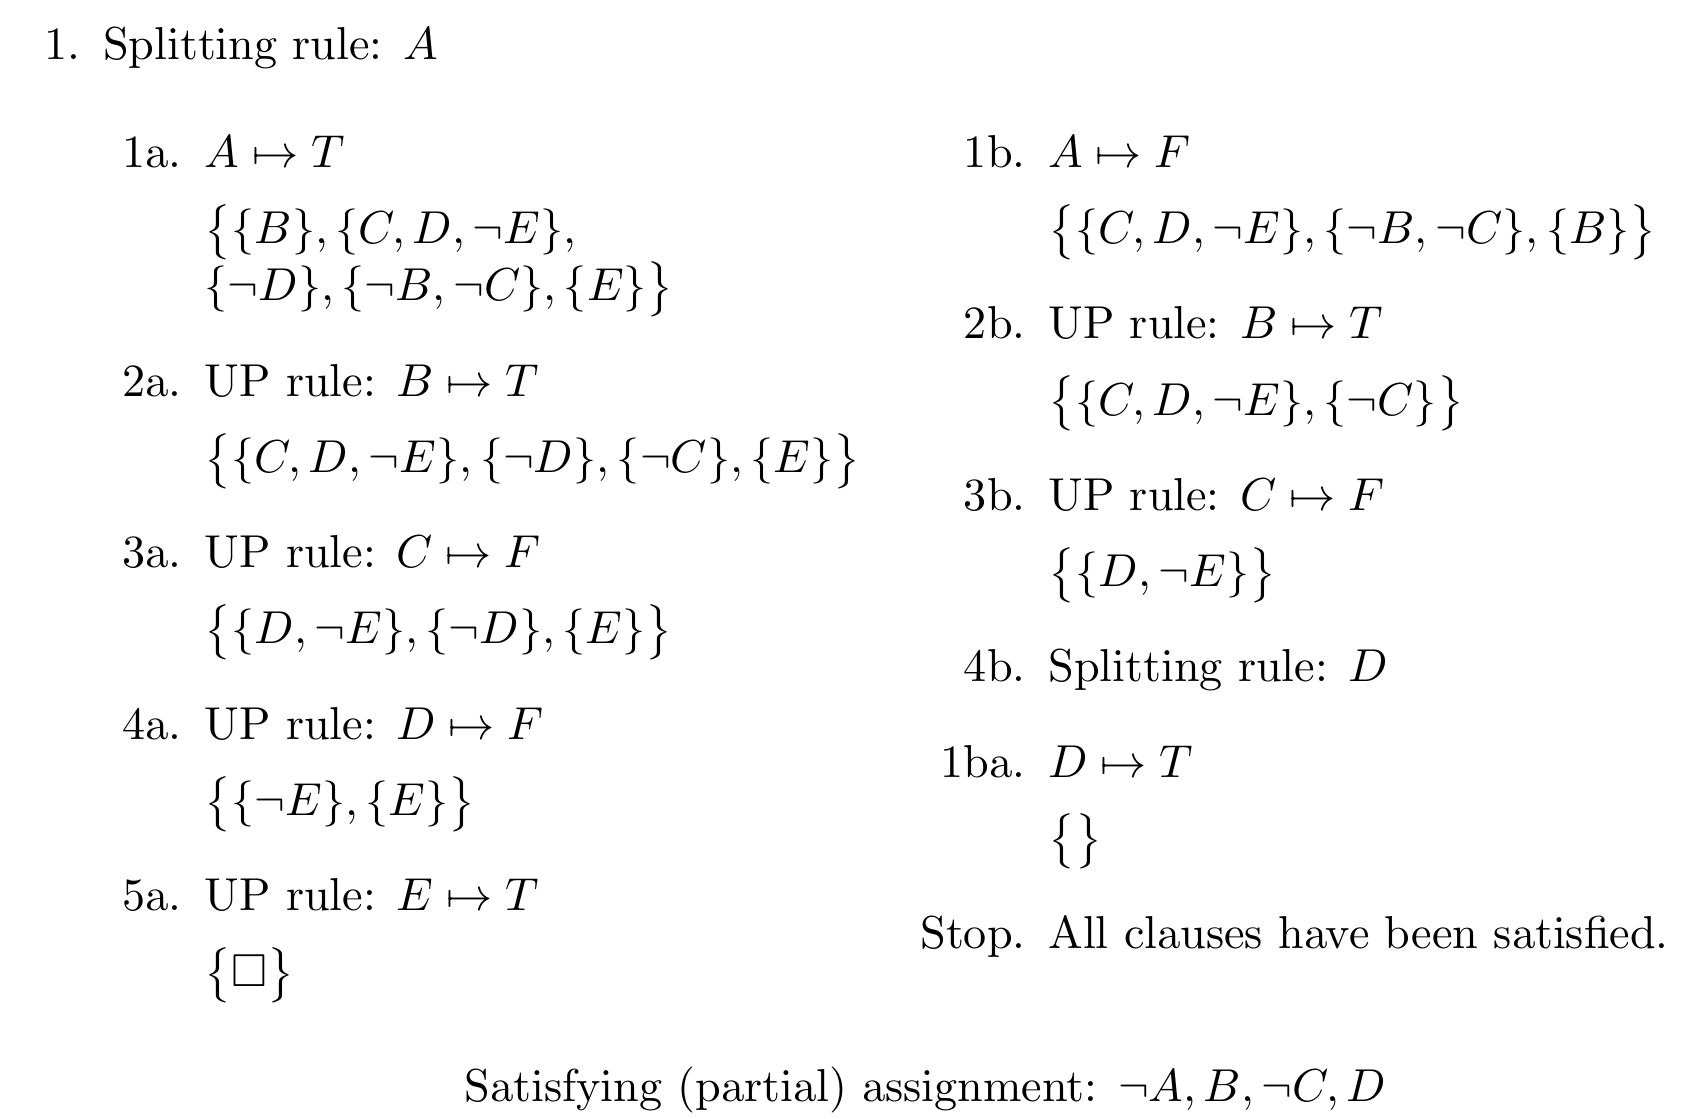
\includegraphics[width=0.8\textwidth]{imgs/dpll.png}

\begin{itemize}
    \item \textbf{this only works for CNF (claused linked with and)}
    \item check for clauses that are small and use splitting rule on them
    \item make sure that you keep going until either the entire set is empty (\textbf{satisfying assignment}) or just a single clause is empty (
\end{itemize}

\subsection{Conflict Graph}

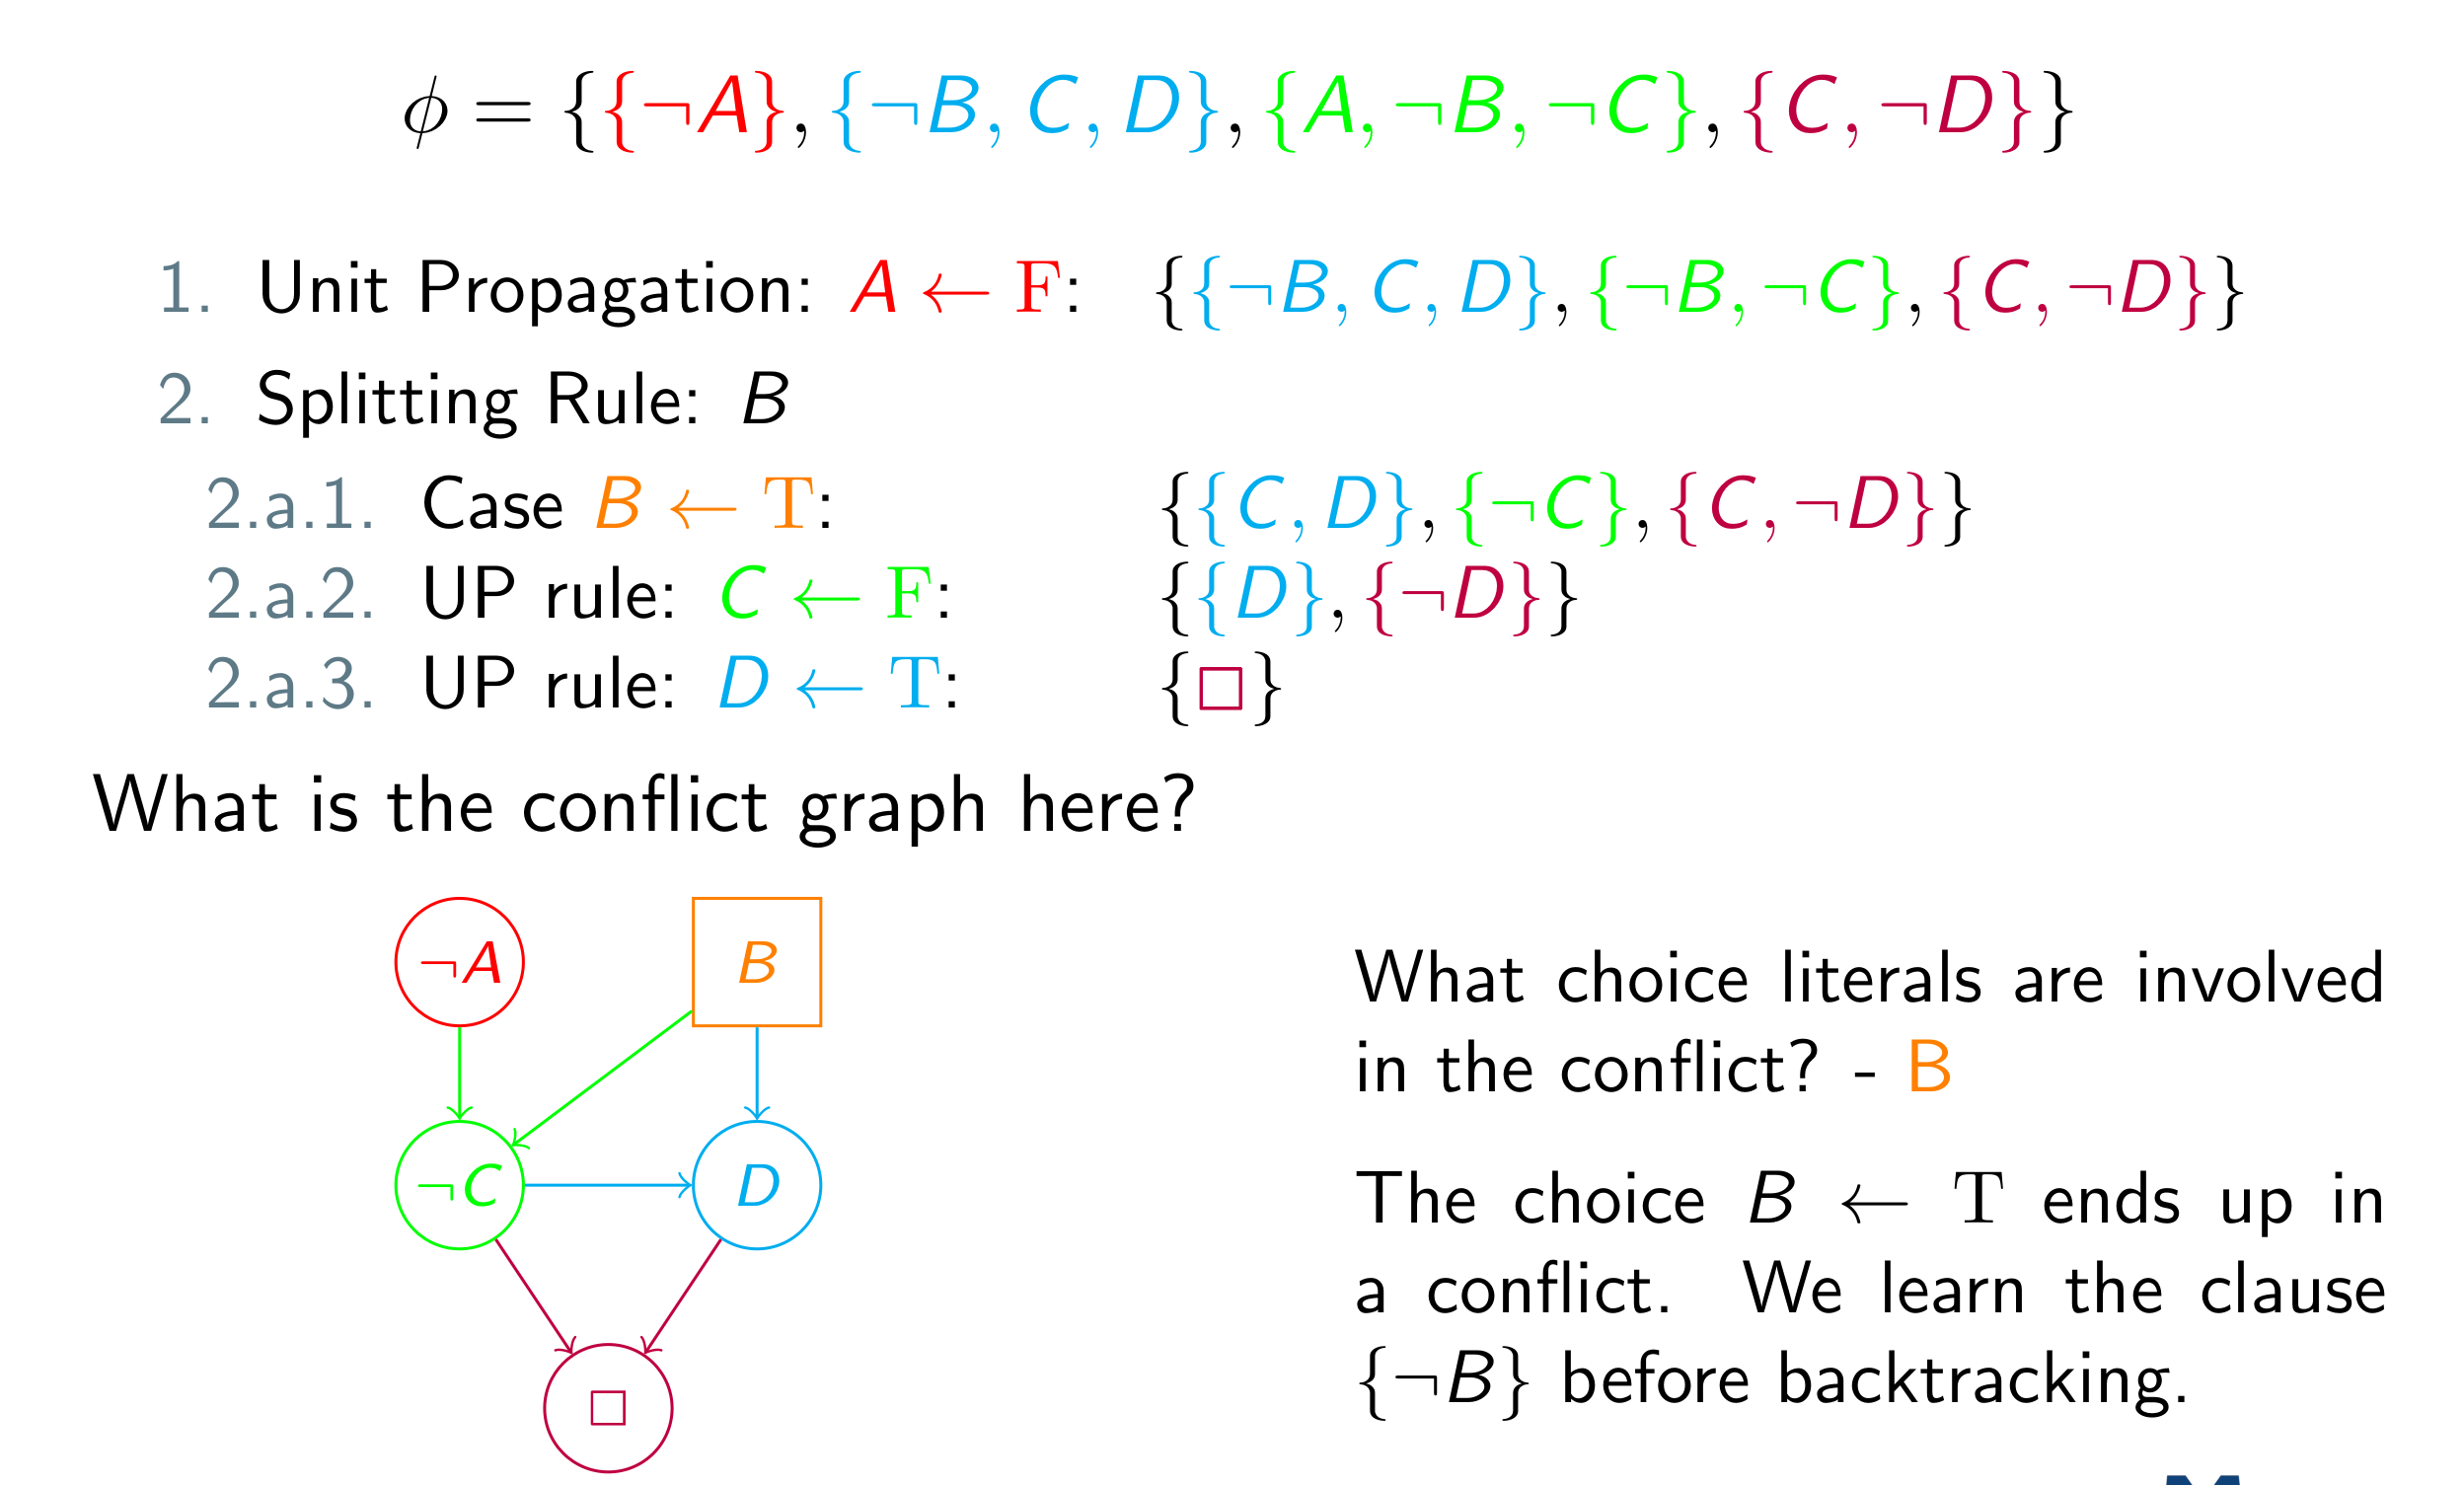
\includegraphics[width=0.8\textwidth]{imgs/conflict.png}

\subsection{Herbrand Christian hat einen wunderbaren Penis Expansion}

\begin{itemize}
    \item can only be used to show that something cannot be satisfied
\end{itemize}

\begin{enumerate}
    \item \textbf{Important! What do we want to reason about?} If the exercise just asks to show that the set of PL1 formulas is unsatisfiable \textit{you can skip this step}, but:\\
    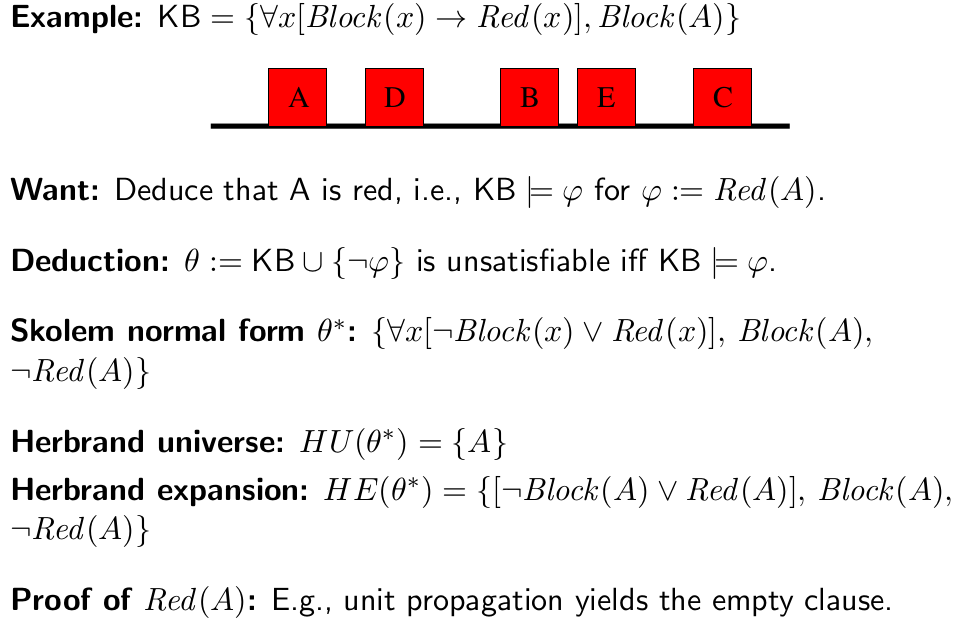
\includegraphics[width=0.7\textwidth]{imgs/herbrand-example.png}

    \item Skolem Normal form: eliminate  $\exists$ and everything else like in prenex normal form:\\\\
    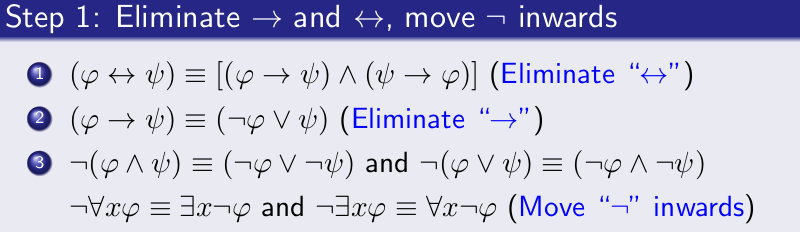
\includegraphics[width=0.7\textwidth]{imgs/step1.png}\\
    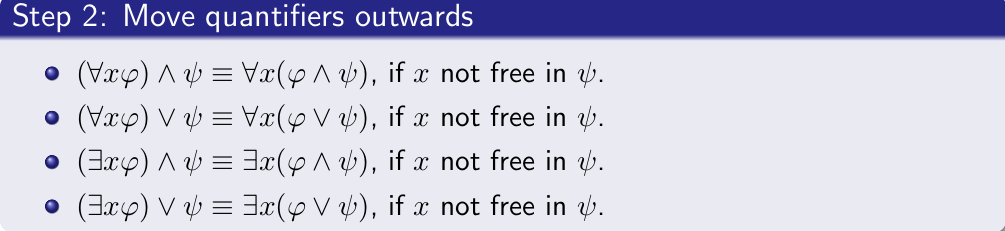
\includegraphics[width=0.7\textwidth]{imgs/step2.png}\\
    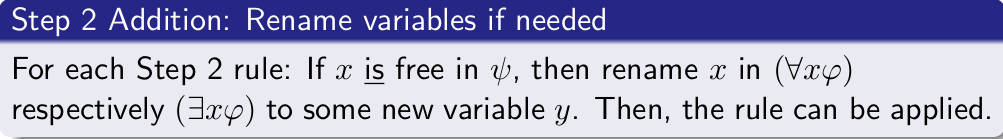
\includegraphics[width=0.7\textwidth]{imgs/step2-add.png}\\
    \item then Skolem normal form:\\\\
    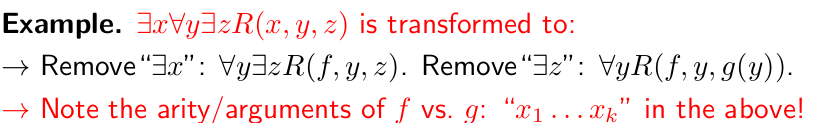
\includegraphics[width=0.8\textwidth]{imgs/skolem.png}\\
    \item put all constants and functions in $CF({\theta}^*) = \{...\}$ and \textbf{if there is no constant} like in $\forall x[\neg Dog(x) \lor Chases(x,f(x))]$ add new symbol c into $CF({\theta}^*)$\\
    \item then the Herbrand universe is built iteratively:\\
    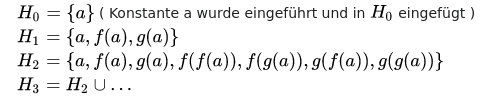
\includegraphics[width=0.8\textwidth]{imgs/herbrand2.png}
    \begin{itemize}
        \item \textbf{all constants are in $H_0$} (example just containts only a)
        \item each iteration applies the functions to the previous iteration to build new terms
    \end{itemize} \vspace{40pt}
    \item now we just instantiate each clause with all terms from $HU({\theta}^*)$ \vspace{20pt} \\ 
    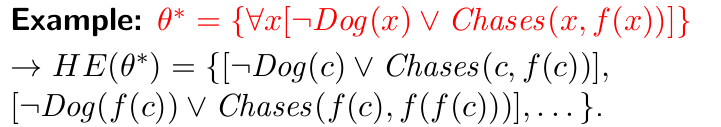
\includegraphics[width=0.6\textwidth]{imgs/expansion.png} \vspace{20pt} \\
    or (from example above) \vspace{20pt} \\
    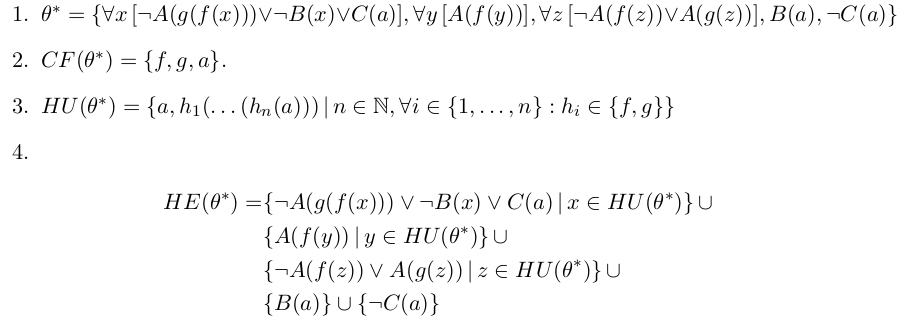
\includegraphics[width=\textwidth]{imgs/expansion2.png} \vspace{40pt} \\
    \item if we want to perform resolution on this universe now, we have to pick elements which will lead to the empty clause, e.g. \\
    
    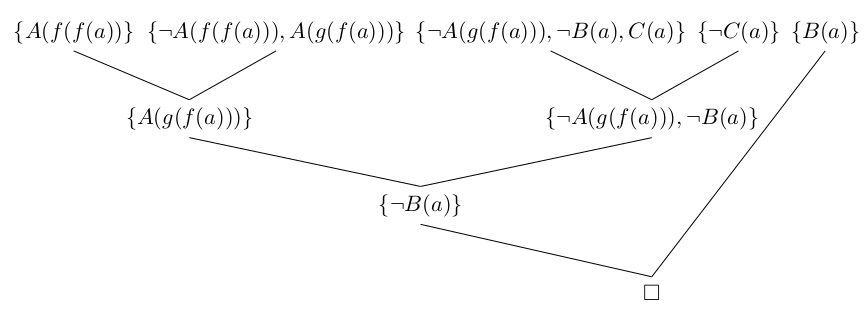
\includegraphics[width=0.8\textwidth]{imgs/resolution-tree.png}\\
    
    Keep in mind that resolution simply follows this rule (we have complementary terms, so we can remove them in the resulting term e.g. $A(f(f(a)))$ and $\neg A(f(f(a)))$):\\
    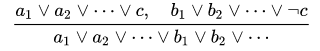
\includegraphics[width=0.6\textwidth]{imgs/resolution-rule.png} \\ %TODO maybe remove this
    
    \textit{Look for terms like $B(a)$, where can potentially obtain two complementary clauses that lead to the empty clause}
    
    
    
\end{enumerate}

\subsection{Unification}

%TODO add more explanations, insights

\begin{minipage}[b]{0.5\linewidth}
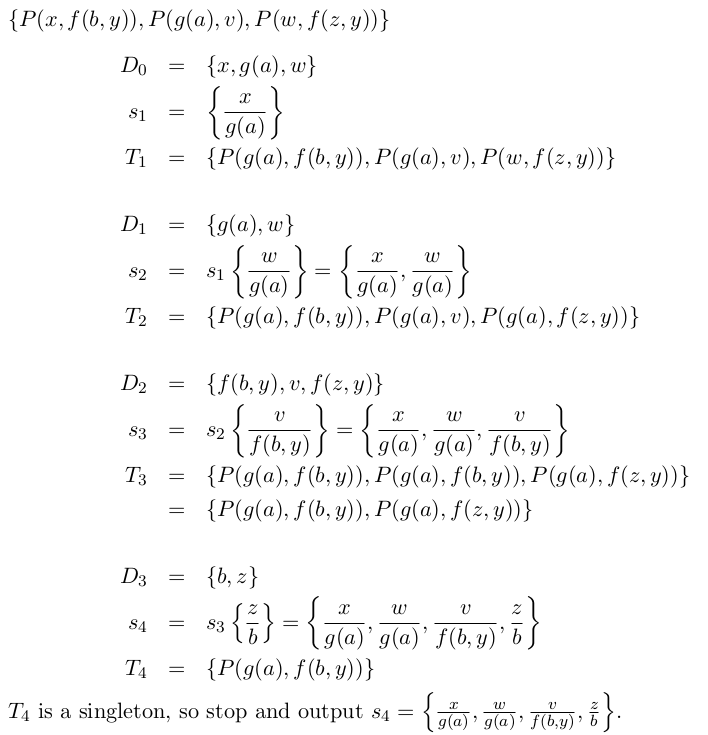
\includegraphics[width=\textwidth]{imgs/unification.png}
\end{minipage}
\begin{minipage}[b]{0.5\linewidth}
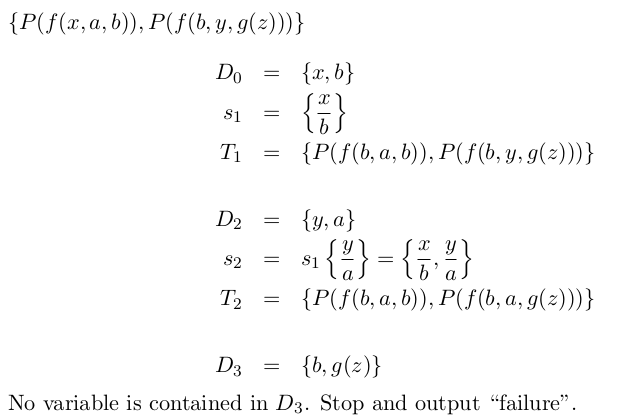
\includegraphics[width=\textwidth]{imgs/unification2.png}
\end{minipage}


\subsection{Binary PL1 resolution (predicates)}

  \begin{minipage}[b]{0.5\linewidth}
  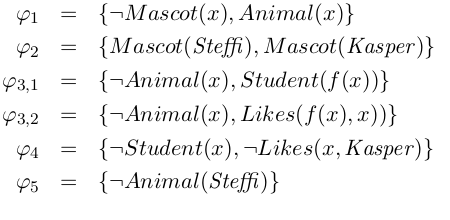
\includegraphics[width=0.8\textwidth]{imgs/clauses.png}
  \end{minipage} 
  \begin{minipage}[b]{0.5\linewidth}
  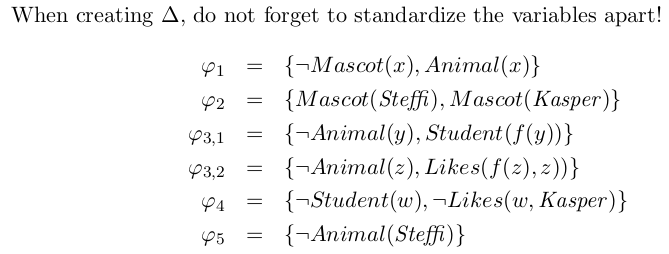
\includegraphics[width=\textwidth]{imgs/clauses2.png}
  \end{minipage}
  
\begin{itemize}
    \item \textbf{do not forget to standardize and transform into CNF!!}
\end{itemize}

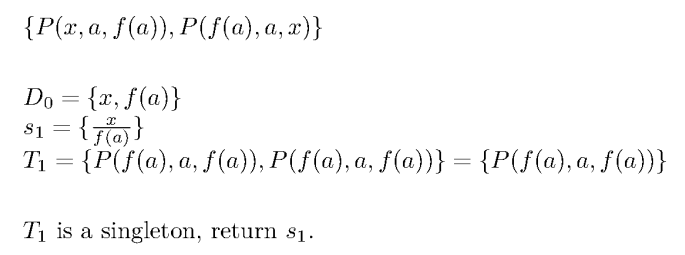
\includegraphics[width=0.8\textwidth]{imgs/PL1.png}

or as tree:

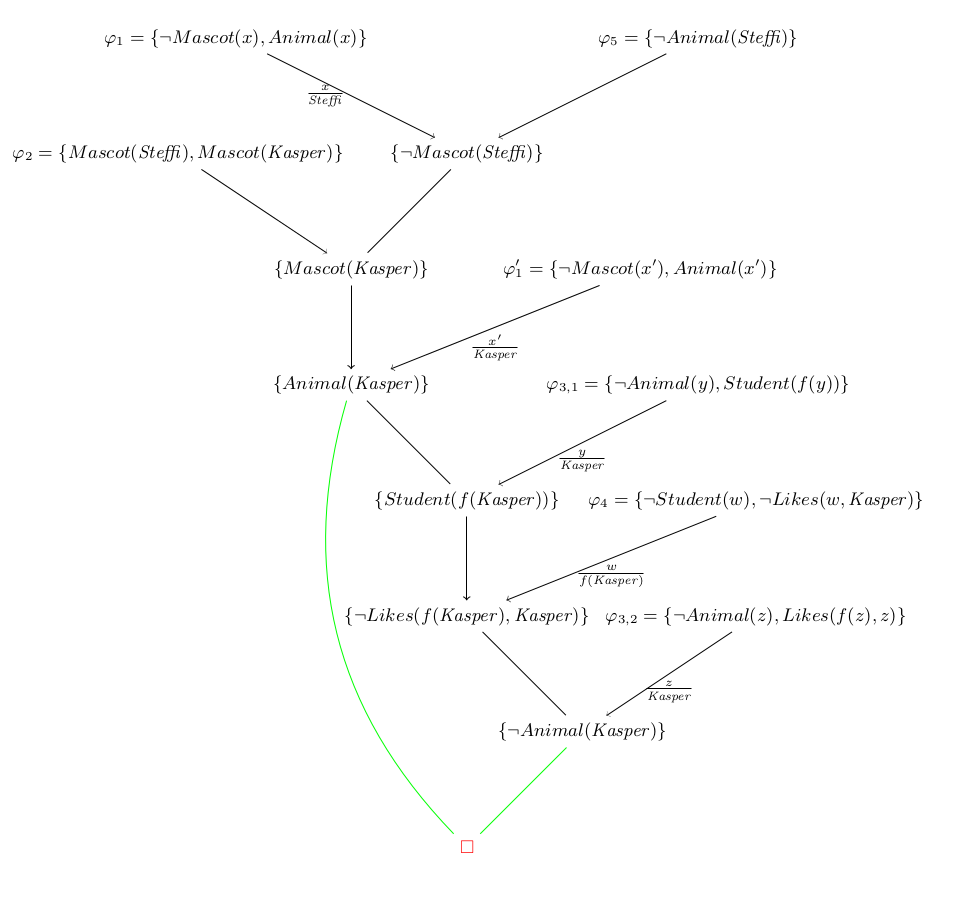
\includegraphics[width=0.8\textwidth]{imgs/pl1.png}

%TODO more about PL1 resolution

\section{Minimax}

\subsection{Search}
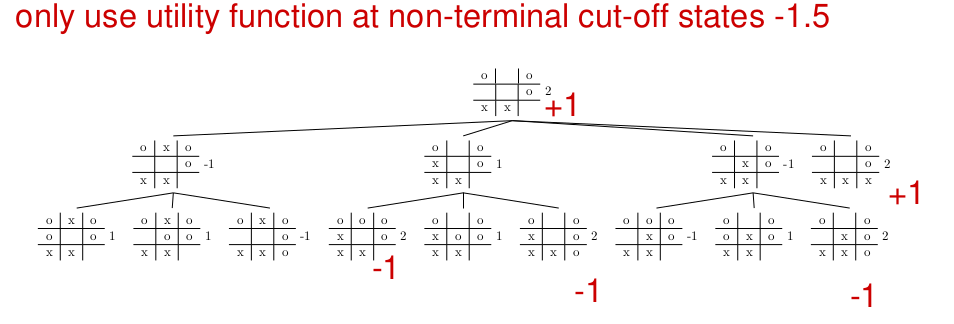
\includegraphics[width=0.8\textwidth]{imgs/minmax.png}

\begin{itemize}
    \item \textbf{make sure to annotate Min and Max on the left side}
\end{itemize}

\subsection{Alpha-beta pruning}

%TODO

%TODO ex. 

\section{A Box/T Box}

\begin{itemize}
    \item make sure that you also specify the inferred assertions if asked ("State all possible A-Box membership assertions of Marge, Lisa and Abraham")
    \item Abraham:Father is a \textit{concept assertion}, (Abraham,Herb):hasChild is not!
\end{itemize}

\subsection{Defining T-Boxes}

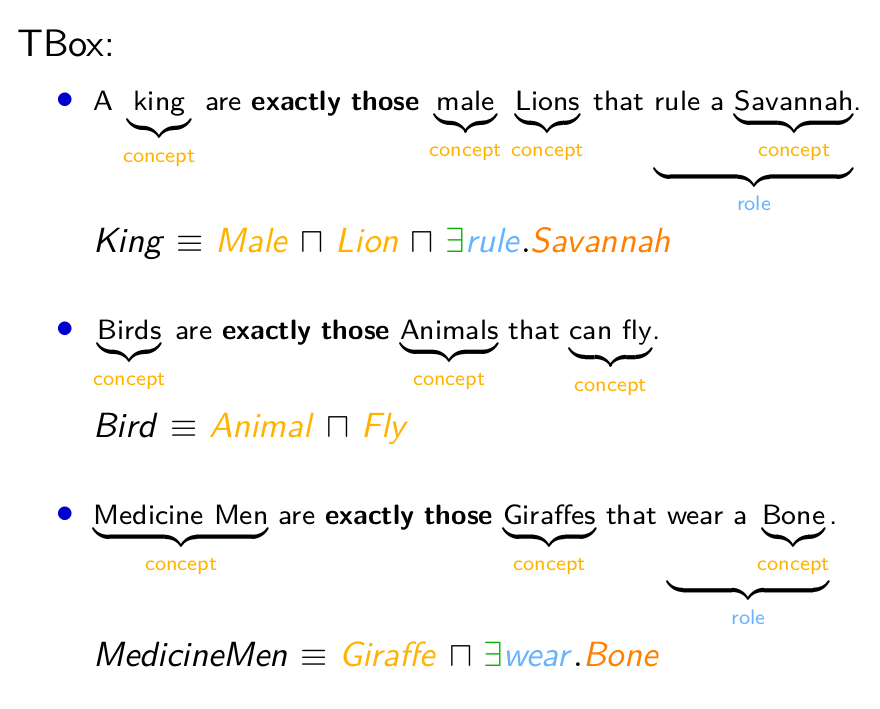
\includegraphics[width=0.5\textwidth]{imgs/tbox-ex.png}
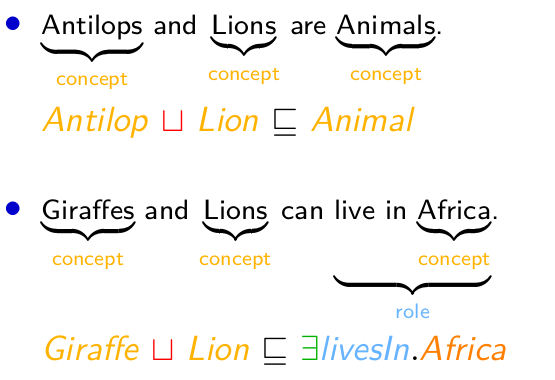
\includegraphics[width=0.5\textwidth]{imgs/tbox-ex2.png}\\
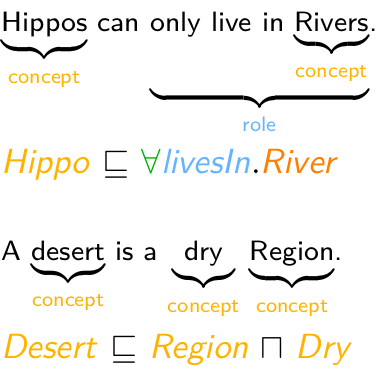
\includegraphics[width=0.5\textwidth]{imgs/tbox-ex3.png}
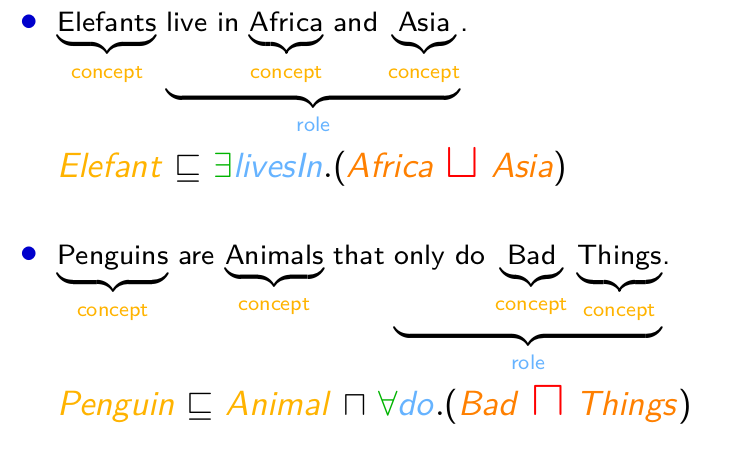
\includegraphics[width=0.5\textwidth]{imgs/tbox-ex4.png}\\

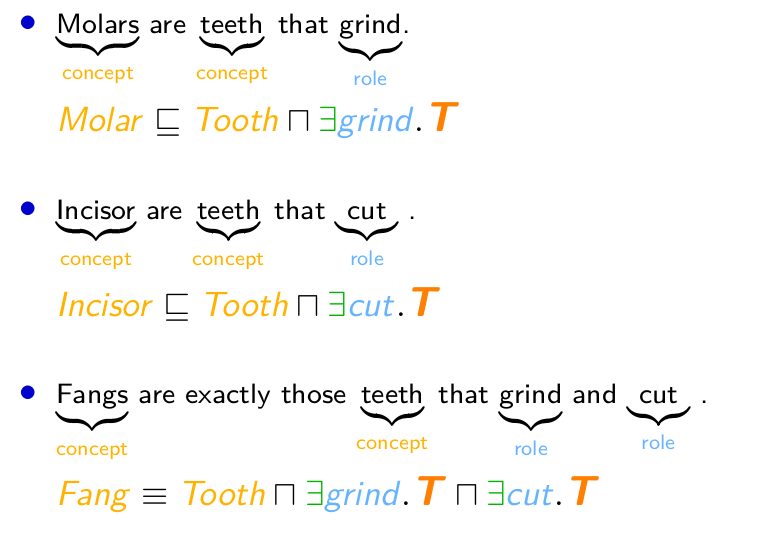
\includegraphics[width=0.5\textwidth]{imgs/tbox5.png}
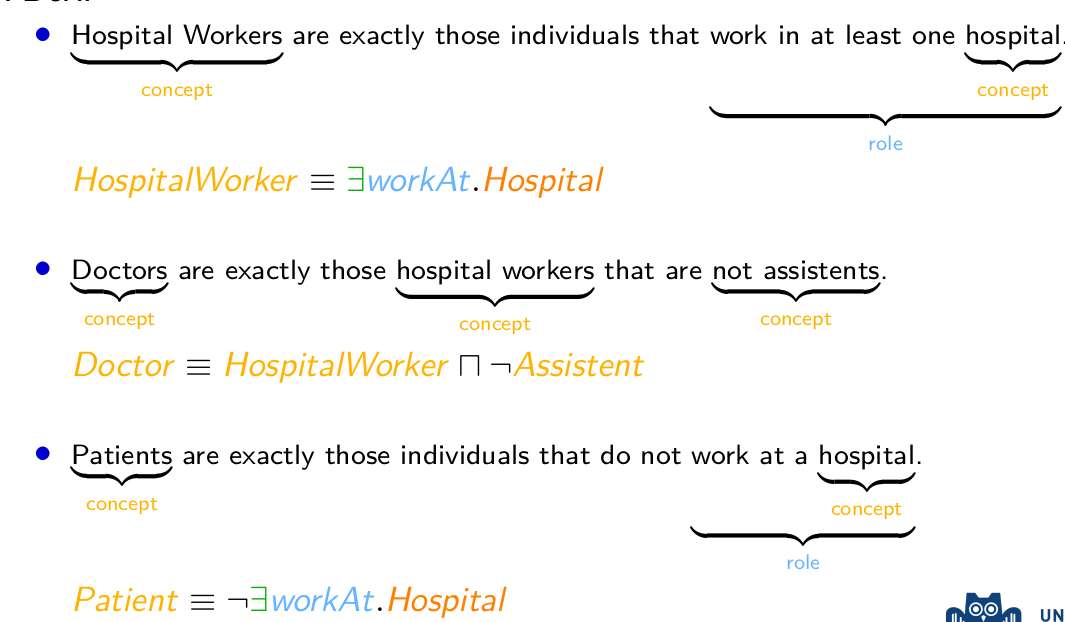
\includegraphics[width=0.5\textwidth]{imgs/tbox6.png}\\
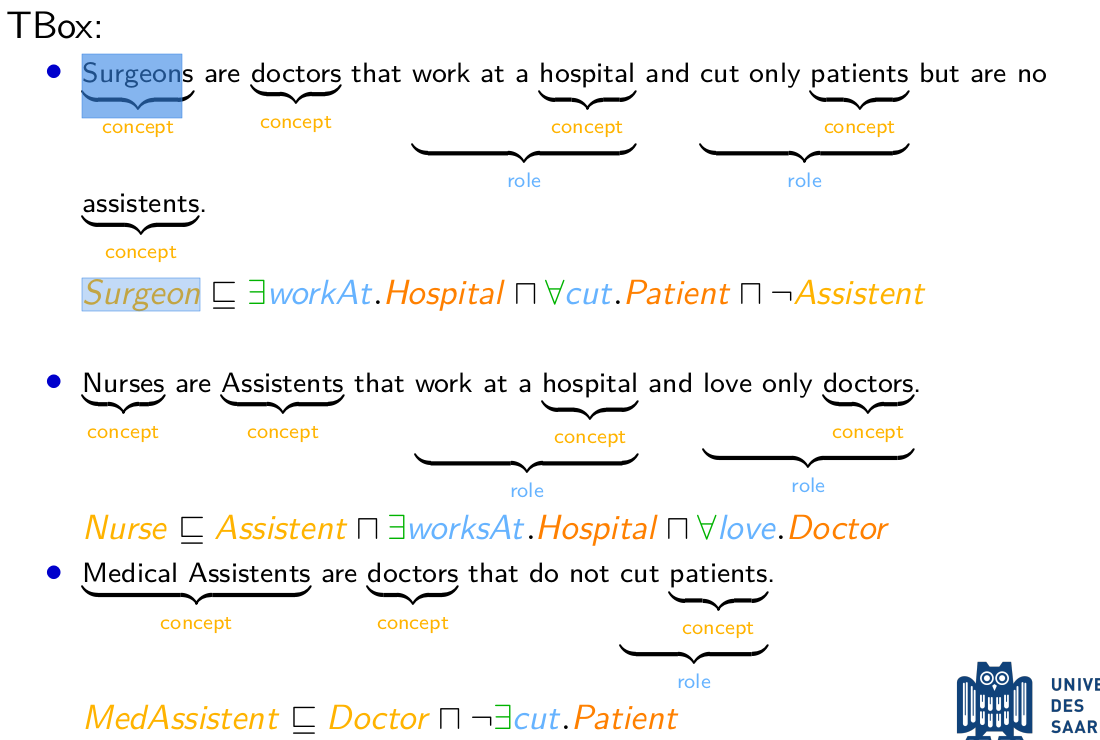
\includegraphics[width=0.5\textwidth]{imgs/tbox7.png}
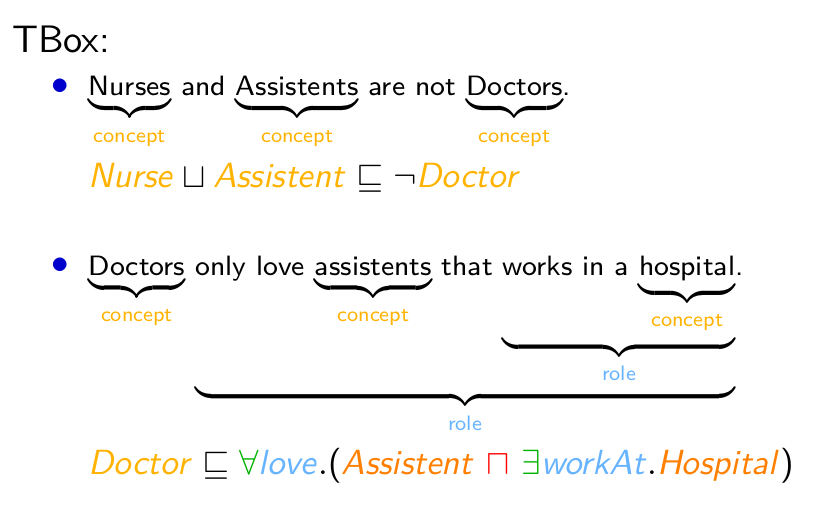
\includegraphics[width=0.5\textwidth]{imgs/tbox8.png}\\

  \begin{minipage}[b]{0.5\linewidth}
  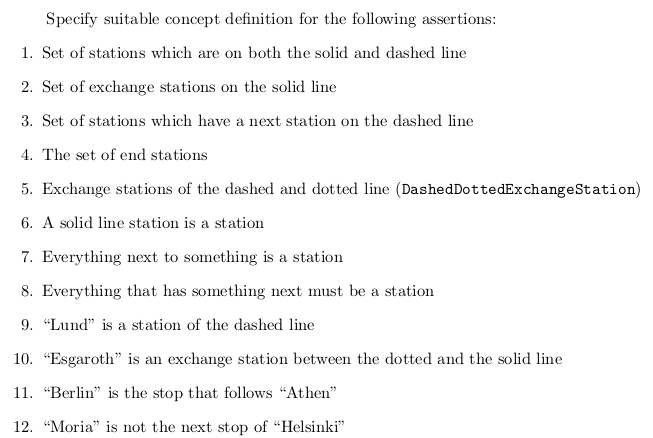
\includegraphics[width=\textwidth]{imgs/assertions.png}
  \end{minipage} 
  \begin{minipage}[b]{0.5\linewidth}
  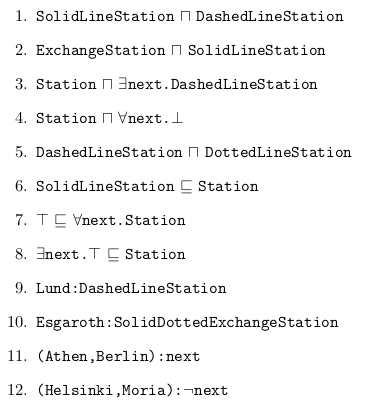
\includegraphics[width=\textwidth]{imgs/assertions2.png}
  \end{minipage}
  
\subsection{Defining A-Boxes}

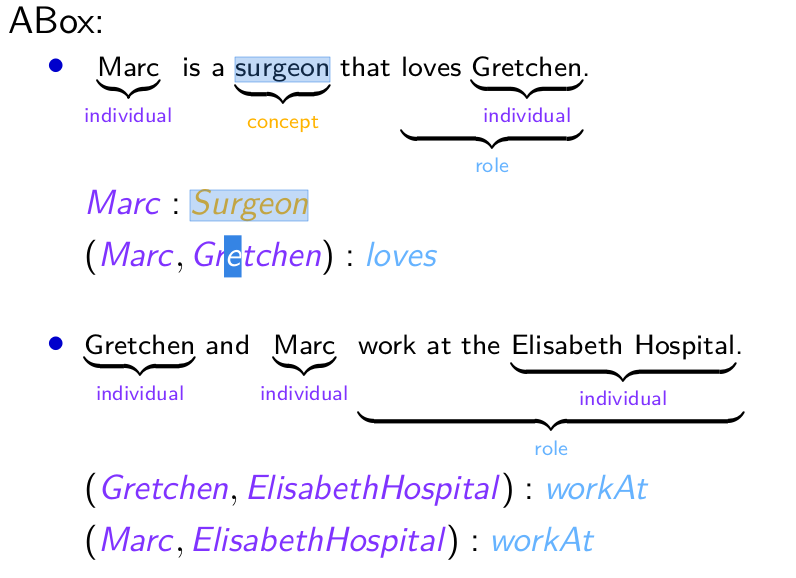
\includegraphics[width=0.5\textwidth]{imgs/abox1.png}
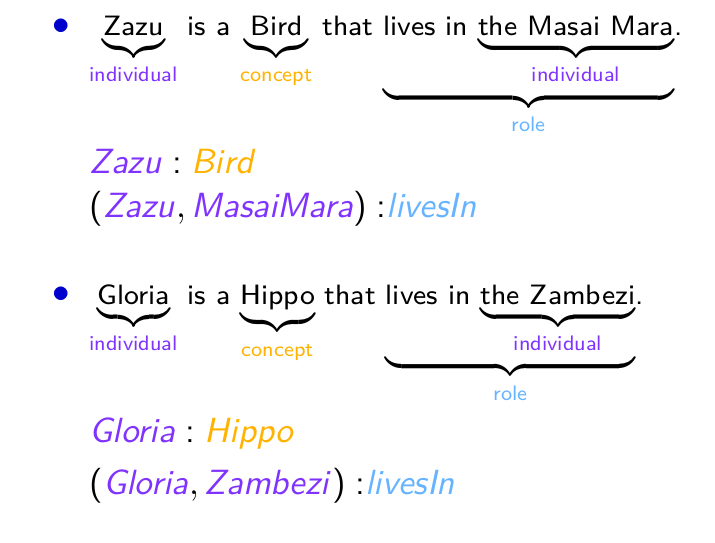
\includegraphics[width=0.5\textwidth]{imgs/abox2.png}\\

\subsection{Visualization}

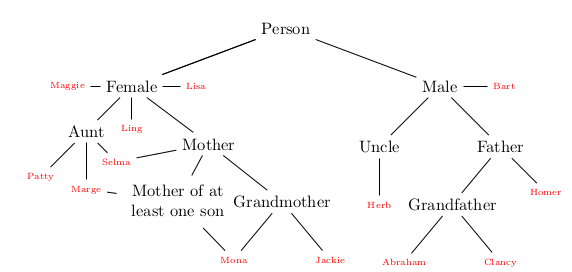
\includegraphics[width=0.8\textwidth]{imgs/tree.png}\\
\subsection{How to prove something with assertions?}
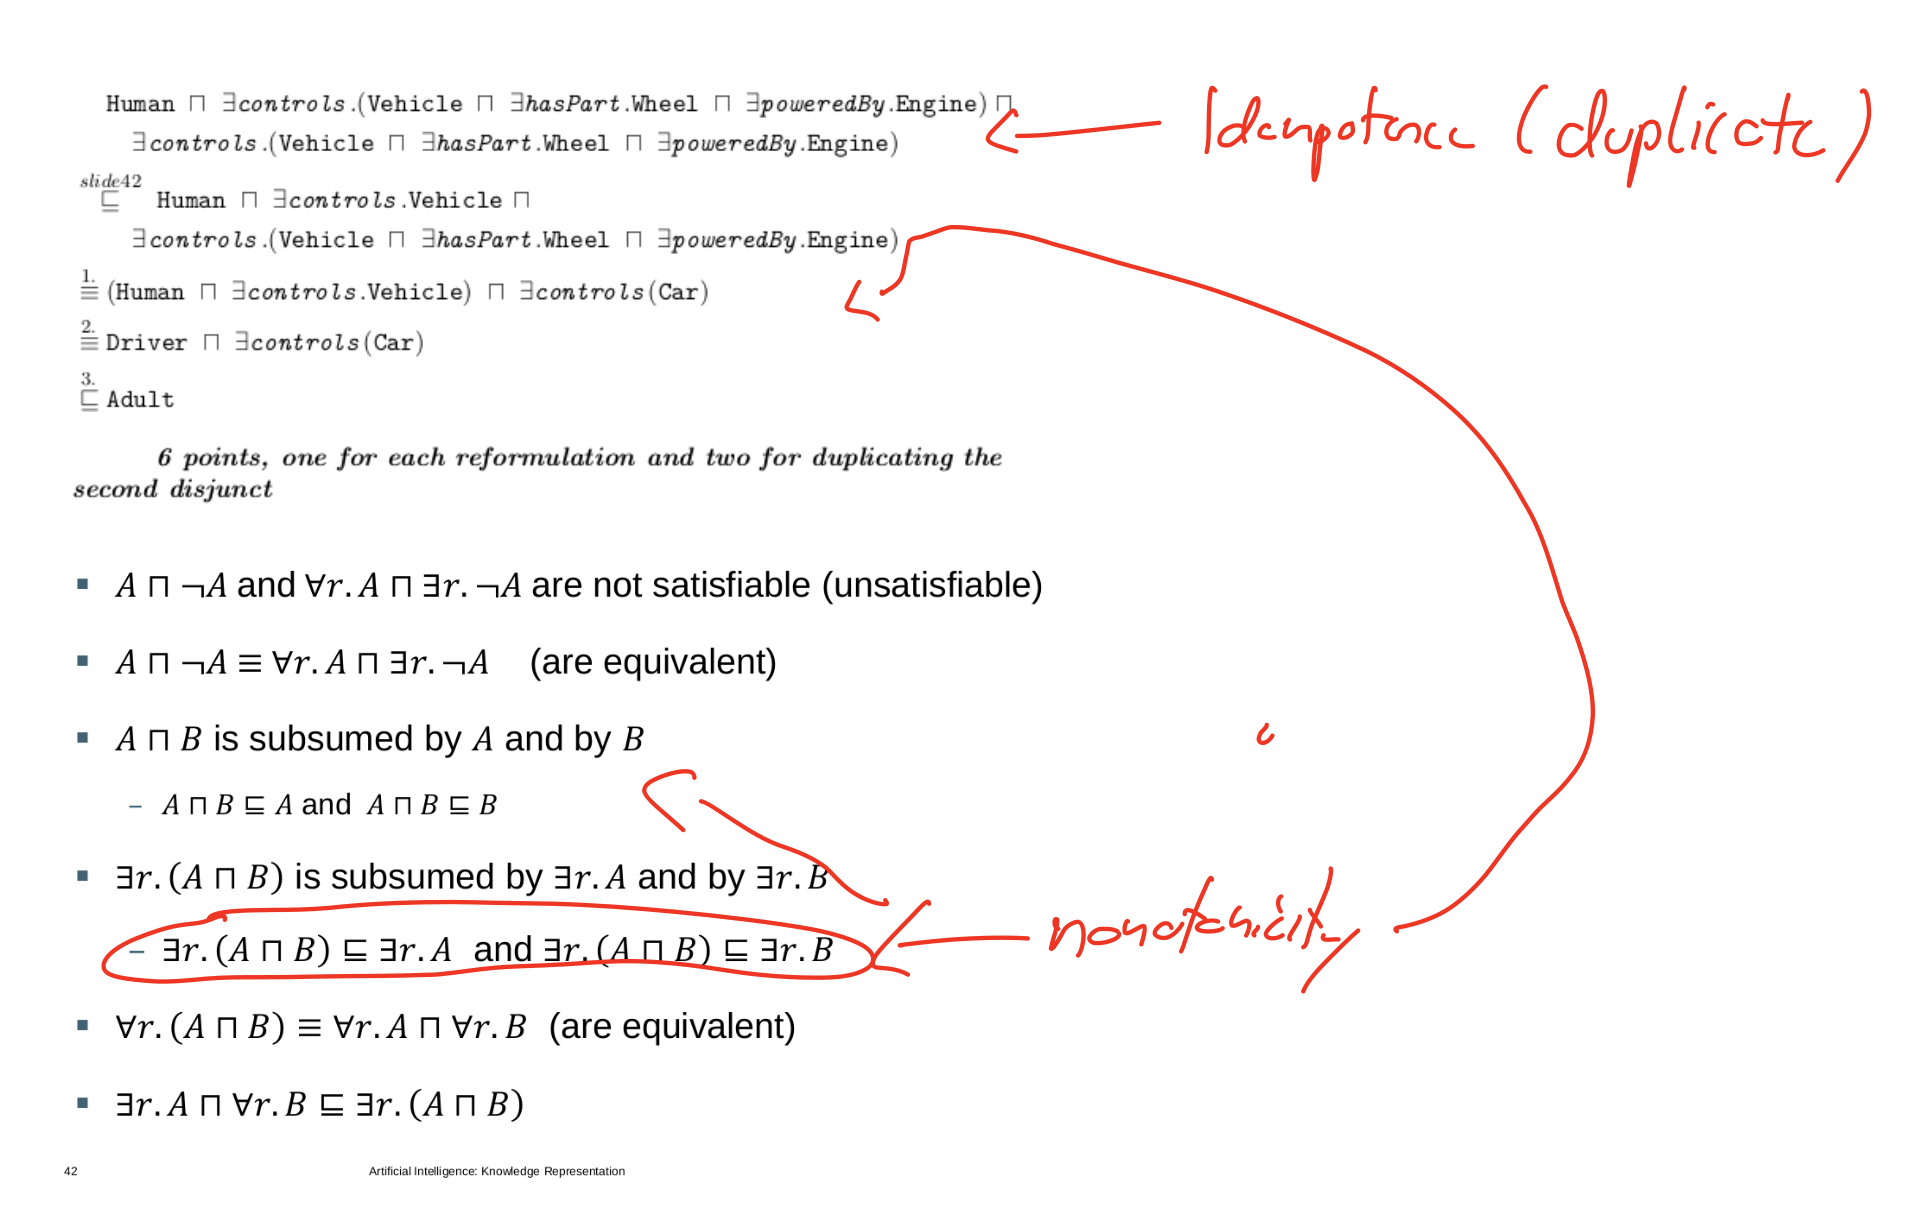
\includegraphics[width=\textwidth]{imgs/equiv.png}
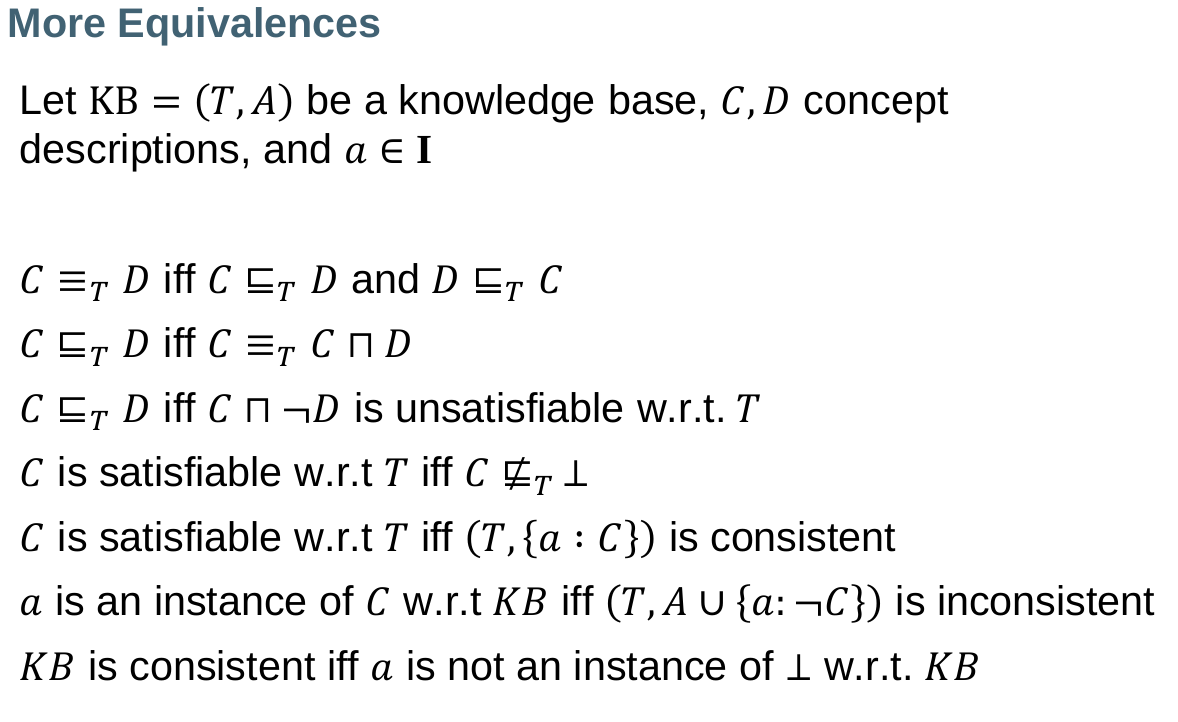
\includegraphics[width=0.8\textwidth]{imgs/equiv2.png}



\section{Naive backtracking}

\section{Formulating a CSP}

\subsubsubsection{Specify the domain}

Here you can define multiple domains at once such as:
$$D_S = D_1$$

%TODO look at it

%\includegraphics[width=0.8\textwidth]{imgs/csp-equal.png}

\subsection{Example: no adjacent pair of the same color}
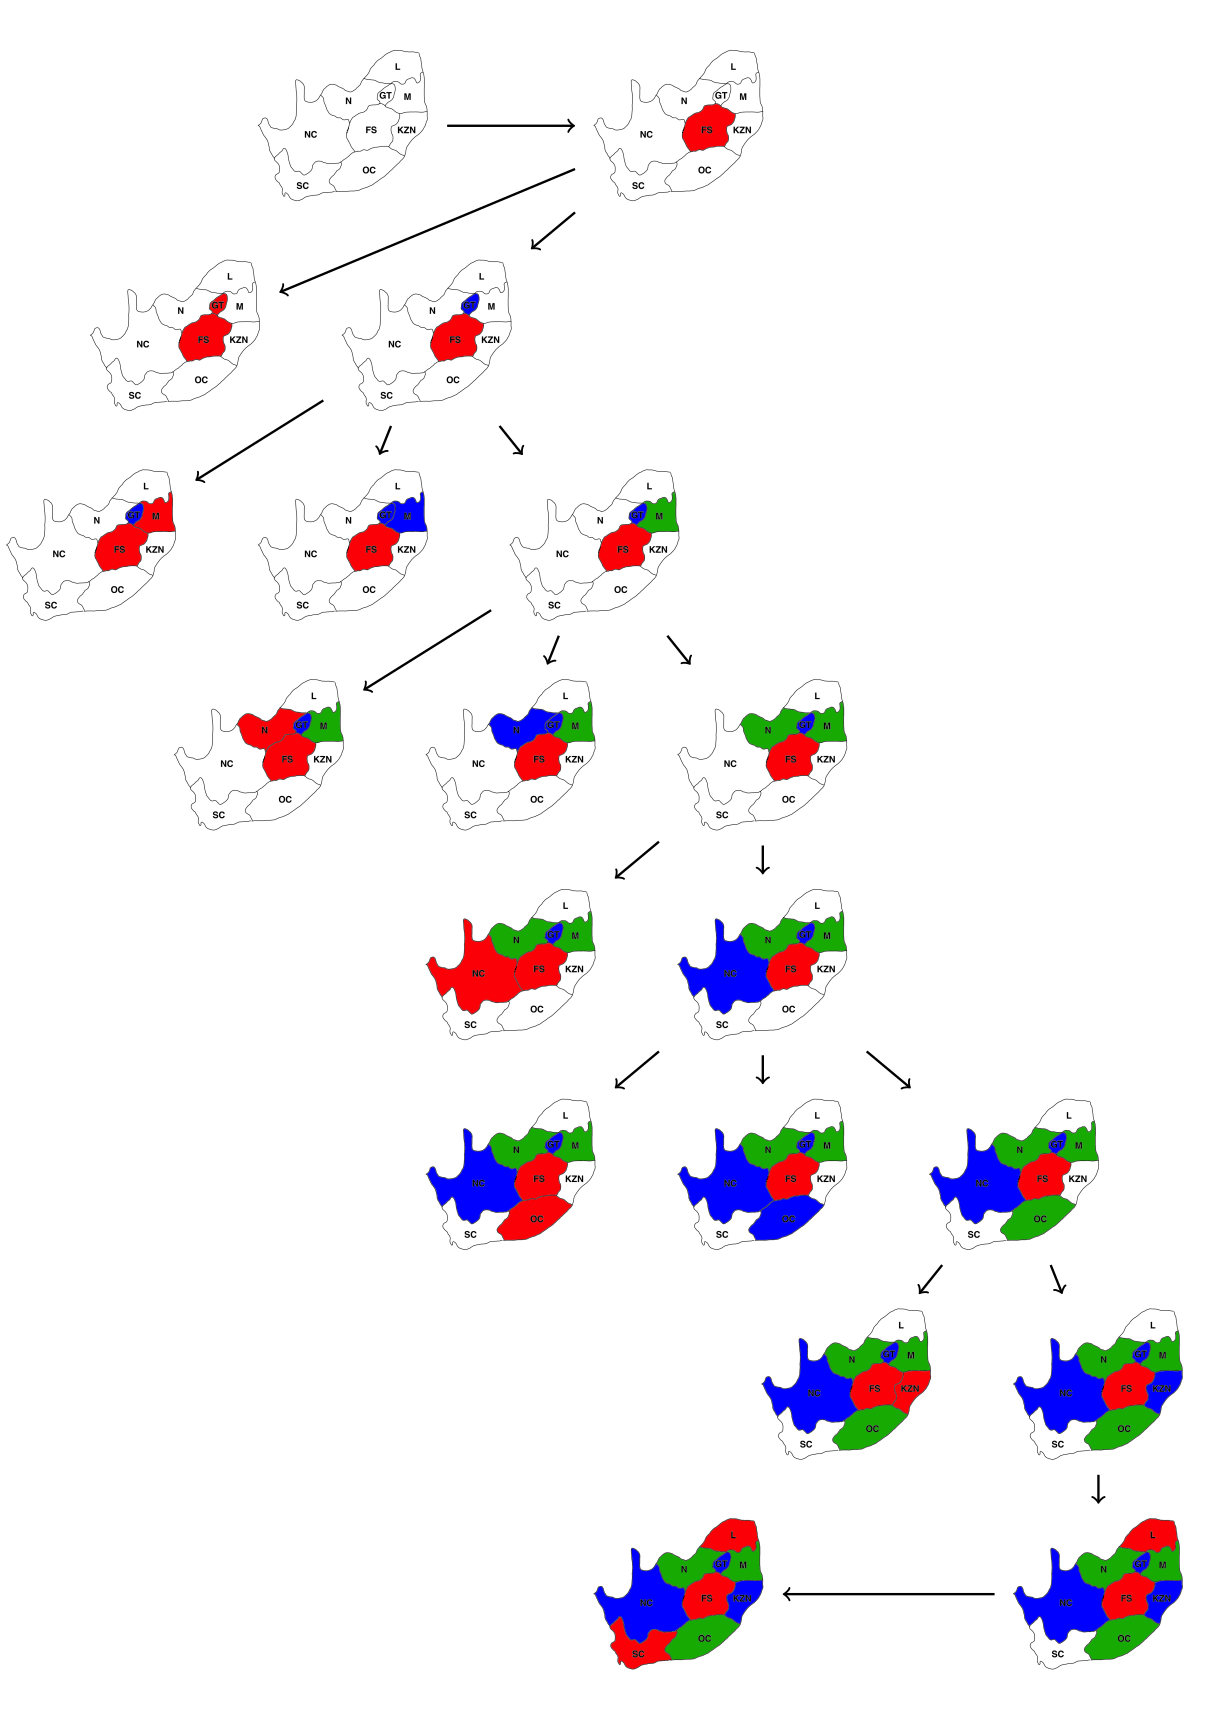
\includegraphics[width=0.7\textwidth]{imgs/naive.png}

\section{AC-3}

\subsection{Constraint graph}

\begin{itemize}
    \item easy, just a graph with the constraints on the edges
\end{itemize}

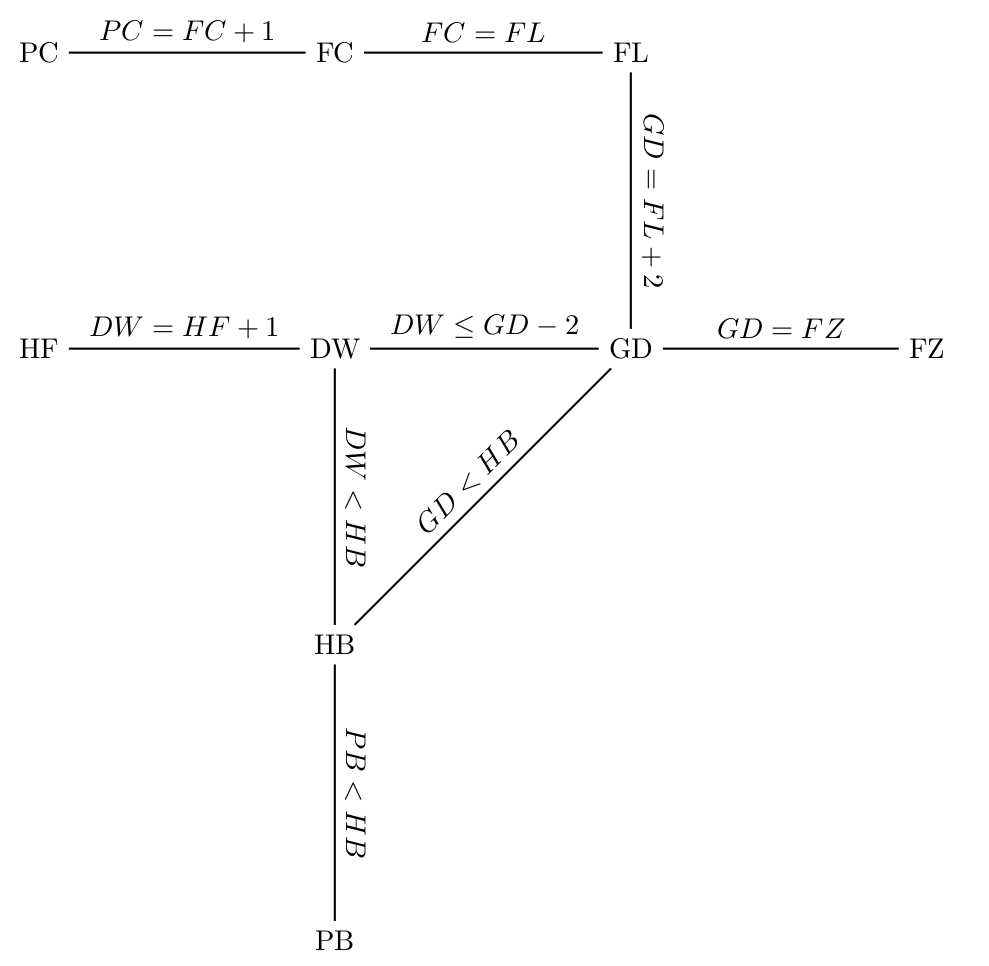
\includegraphics[width=0.7\textwidth]{imgs/constraint.png}

\subsection{Run the algorithm}

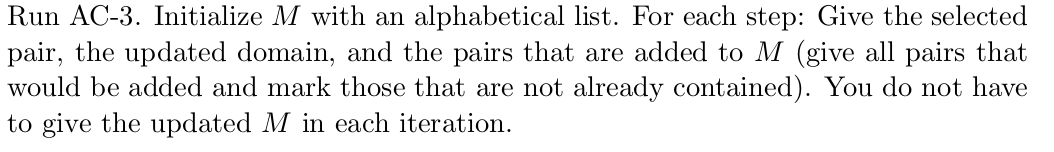
\includegraphics[width=0.8\textwidth]{imgs/ac-3.png}\\
\includegraphics[width=0.8\textwidth]{imgs/ac-32.png}

\begin{itemize}
    \item \textbf{add the transitive pair for all constraints even $FC=FL$}
    \item check if you also have to add pairs that are still contained (''give all pairs that would be added and mark those that are not already contained'')
    \item What happens during each iteration?
    \begin{itemize}
        \item alphabetical list $\implies$ priority queue!!!
        \item \textbf{We only restrict the domain of the left part of the tuple}
        \item Keep in mind what the domains of the two variables are
        \item If it is supposed to be ordered alphabetically 
        \item if the queue is \textbf{empty} we return the modified domains\\
        \includegraphics[width=0.5\textwidth]{imgs/result.png}
    \end{itemize}
\end{itemize}

\section{Acyclic-CG}

\subsection{Draw the directed tree (Pick DW as root and remove DW < HB)}

\includegraphics[width=0.5\textwidth]{imgs/tree2.png}
\includegraphics[width=0.5\textwidth]{imgs/constraint.png}

\subsection{Variable order (step 2 of the algorithm)}

\begin{itemize}
    \item DW, GD, FL, FC, FZ, HB, HF, PB, PC (example)
\end{itemize}

%TODO variable ordering


\subsection{List the calls to $Revise(\gamma, v_{parent(i)}, v_i)$ and give the resulting domain of $v_{parent(i)}$}

\includegraphics[width=0.5\textwidth]{imgs/revise.png}

\begin{itemize}
    \item so we start with the last variable in the order first (since the algorithm iterates beginning with n, not 1)
\end{itemize}

\subsection{BackTrackingWithInference}

%TODO


\end{document}
